\documentclass[a4paper, 12pt]{book}

\usepackage[utf8]{inputenc}
\usepackage{blindtext}
\usepackage{graphicx}
\usepackage{pgfplotstable}
\usepackage{booktabs}
\usepackage{filecontents}
\usepackage{longtable}
\usepackage[T1]{fontenc}
\usepackage[backend=biber]{biblatex}
\addbibresource{references.bib}
\usepackage[skip=5pt plus1pt, indent=0pt]{parskip}

\usepackage[hidelinks]{hyperref}
\hypersetup{
    linktoc=all
    allcolors=black
}

\graphicspath{ {./images/}{./troubleshooting/crumb-structures/} }


\title{%
  The Sourdough Framework\\
  \large How to master making bread at home\\
  \small - the bread code community book -}

\author{Hendrik Kleinwächter}
\date{\today}

\begin{document}

\begin{titlepage}
\maketitle
\end{titlepage}


\frontmatter

\tableofcontents

\chapter{Foreword}
Still need someone to write a foreword

\chapter{Preface}
If there is one food Germany is known for, it is probably bread.
There are thousands of varieties in Germany,
and making it has been an integral part of our culture.

My bread journey began during childhood. My mother, being a parent
of 3, would always use Saturdays to bake a delicious loaf for the family.
It was a white fluffy sandwich bread, and she made it within one to two hours using store-bought yeast.
Being a bit more experienced, I now realize it's
ideal to wait a little while before cutting into your bread, but back then,
we kids couldn't wait. Mom would cut for us a few slices straight from the oven, and we would
immediately proceed to pour butter or jam on each slice. Within minutes, 1kg of
flour would be consumed. Bread became an integral part of my weekly food.

I was lucky that my parents could afford a yearly ski trip to
Alto Adige in northern Italy. In the small town called Valdaora, we
would try new restaurants every year, yet always end up in our favorite
pizza place. The pizzas there were incredible. The dough
alone was so tasty that we would order just the bread with a
bit of olive oil and salt.

Of course, my question would always be, ``Mom, can we make this at home, too, please?''
So over the years, we became friends with the owners and would receive
more and more clues as how to make the perfect pizza dough. There
are no secret ingredients inside. It's just flour, water, salt, and a bit of yeast.
How can such a simple combination of ingredients create such an incredibly delicious
pizza dough? My parents, being creatures of habit, would return every year with us,
and every year, my interest would grow. At home, Mom and I attempted to replicate
the recipe. We tried baking on a stone and on a steel. We tried adding oil to the dough and herbs
to the pizza sauce. We fell into an endless cycle of experiments. However, we never managed
to get close to the experience we had while on vacation.

Some years passed, and I eventually began my studies in the small German city of Göttingen.
For the first time, I was faced with shopping for my own bread. It was never
on my mind to actually start baking it for myself. I would just buy 
a good loaf while shopping at the supermarket. My favorite variety
was a Schwarzbrot, Korn an Korn. It’s a very dark and hearty rye bread
with added berries and sunflower seeds. Being a little naive,
I'd never before examined the packaging of what I was buying. One day, that
changed.

I looked at the label and was shocked. The seemingly
healthy bread consisted of so many other things aside from flour and water.
The black color was not coming from the flour, but from caramelized sugar.
The packaging stated it was a sourdough bread, but then why was there additional yeast?
I thought that if it was really sourdough, it shouldn't require additional yeast, and I
soon realized that something was wrong with the bread I was buying.
I proceeded to check the other supermarket breads, only to discover that they, too,
contained ingredients I'd never heard of. That was the day I lost trust
in supermarket bread.

At home, I decided to research the proper way to make bread, and much to my surprise,
I learned that the recipes for making pizza and bread were actually quite similar, yet
there were also diffferences. For example, some recipes would call for fresh yeast, while
others would call for dry. Deep diving into various online forums and all their many
discussions, I became even more confused.

I tried using different flours and different brands, all in both organic and non-organic varieties.
I realized then that I knew nothing about making bread. Recipes would often contradict each other,
leaving me further confused. They seemed like little more than a collection of apparently random
steps to follow. The baking instructions and temperatures were all different, too.

Meanwhile, having completed my studies, I started work as an engineer.
We engineers are faced with many challenges. The compiler or runtime is
always screaming at you with errors, and it's your job to figure out how to fix them.
It can take hours, sometimes days just to fix a simple problem. If you want
to become a software engineer, you have to develop a certain ``never-give-up'' attitude.

Frequently when writing code, a set of pre-made routines are required. These routines have been
written by other engineers and can then be used to ship code faster.
This pre-written code is commonly known as {\it a framework}. In many cases,
these frameworks are not built by a single person but by engineers from all around the world,
each of whom can help by improving and changing the source code. Frameworks have made many successful
businesses possible.

In most cases, frameworks do exactly what they claim they do. However,
sometimes you are faced with issues you don't understand. In 99.95 percent
of all software bugs, the developer is the issue. Sometimes, however, the framework has a
bug. That is when the developer must dig deeper to see the what and the why behind what the
framework is doing. You will need to read other engineer's source code, and you will be forced
to understand {\it why} things are happening.

Being unhappy with what I was baking, my engineering mindset took over and I had
to do my own deep dive to understand what was going on. Much to my surprise, however,
none of the recipes I'd encountered would tell me {\it why} I should use amount X
of water and amount Y of flour, or {\it why} exactly I should use fresh yeast over dry yeast. Why
should I slap my dough while kneading it on the counter? Why is a standmixer
better than kneading by hand?  Why should I let the dough sit for this long?
Why is steaming the dough during baking important? Do I really need to
get myself an expensive dutch oven to bake bread?

The problem compounded when I started reading about sourdough. It all sounded like black
magic. Why were some sourdoughs made from fruits, while others were made from flour?
Why should one recipe use wheat while another used rye or spelt? How often should the
sourdough be fed? The questions I had then could have filled 20 pages. I was confused,
but became even more determined to learn how decent bread should be made at home.

The feedback I received from friends helped me to improve with each
iteration of homemade bread. Compared to coding, where you sometimes have to wait months
for this feedback, bread making is much more direct. Plus, you can eat your successes
(and failures!) And, much to my surprise, even those failures started tasting better than
most store-bought breads. Eating a homemade bread that takes you hours to make allows you
to develop a different relationship with your food, and baking bread from scratch with my
bare hands was a welcome change after hours of working on the computer.

I continued learning about the process of fermentation and various techniques of bread making.
I approached the topic of sourdough in a manner similar to software, and after years of
researching and documenting my progress, I decided it was time to share that progress with the
world.

When working on open source projects, it is important to see their history and how the source
code changes over time. This way, you can easily jump back to previous versions. This was
the perfect tool for documenting my recipes, because they, too, would change with each
subsequent iteration. Much to my surprise, my open source work on sourdough was appreciated
by other engineers, and the project became popular on the website GitHub, originally built to
share open source software.

Now, when baking great bread, you also need to learn certain techniques. I figured it would be
easier to share these techniques in video form. Thus, my YouTube channel was born. I chose
the name {\it The Bread Code} to capture my engineering-oriented approach to bread. It took some
time to get right, but after choosing more engaging thumbnails and titles for
the videos I made, the channel started gaining viewers.

Now, three years later, I dedicate two days each week to follow my bread baking passion, while
the other three days I continue to work as a software engineer, writing code on a day-to-day
basis.

My bread days fill me with both joy and passion. To me, there is nothing better than seeing
how many people have made amazing bread thanks to my tips and explanations. The community has
continued to grow, spawning many interesting discussions and ideas surrounding the topic of
bread making. There is always something new to learn, and I feel that even now I am just barely
scratching the surface with what I know and teach. Would you ever have imagined that fruit
flies are like bees and are part of the wild yeast's success story? I made a video where
I tried to cultivate wild yeast spores coming from fruit flies in order
to bake bread. It worked; the bread turned out amazing and even tasted good! These kinds of
experiments spark my natural interest. Conducting them and seeing how other people share in my
interest makes me incredibly happy.

The problem with running a YouTube channel is that all the information
you see is filtered and then provided to you through an algorithm. I am concerned
with how algorithms are shaping modern information, because they tend to
put users into certain categories where they will then only see news related to
those same fixed categories. A key metric determining visibility of your channel is how many
people have clicked on a video after it's been shown, and the content you create
is not even shown to every subscriber of your channel. If the algorithm determines the video
is not engaging enough, your content starts to decay in YouTube's nirvana. Even if your video
goes viral, the algorithm will stop showing it once engagement rates with new users goes down,
and older videos fade over time as the decay punishment factor increases. I know, because
I have developed similar algorithms myself as a software engineer.

I've since decided to take some time off from the algorithm cycle to work on something more
long term and meaningful. My mission has always been to share my knowledge with as many people
in the world as possible. That's also why my content has been provided in English rather than
German. After discussing with members of the community, I figured that writing a book could
help me achieve that goal. Most of the books that exist today are collections of recipes. My
idea, however, is to provide you with a deeper foundation of knowledge that you can use to
follow other recipes.

In software terms, this would be a {\it bread framework}.

It is my goal for this book to help everyone facing issues with flour, fermentation, baking,
and more. It should provide a detailed understanding as to why certain steps are necessary
and how to adapt then when things go wrong while making bread.

It is my desire for this knowledge to be accessible to everyone around the world, regardless
of budget, and as such, do not want to charge for the book. That's why I've decided to make
it open source and have asked the community to support my work financially via my ko-fi page
(https://ko-fi.com/thebreadcode). The community's feedback has been amazing so far, and
I've already raised much more money than initially expected.

The first version of the book will only be available digitally---this way, everyone can read
it---though there might also be a hardcover version in the future, depending on how well received
and appreciated it is by bakers around the world. The hardcover version will, of course, cost a
bit of money, but the digital version will remain free.

In this book, I will try to be as scientific as possible. I in no way claim, however, that
it will itself be a work of science. I have conducted several experiments that I will write
about here, but to truly call this science, you would probably need to repeat the same experiment
a thousand times in a lab environment, which I have not done. I will do my best, however, to provide
scientific references where possible and to clearly distinguish between facts and personal opinion.

I hope you have fun reading this and that you learn more about the fascinating world of bread
making, and it is my sincere wish that this work provides you with the solid toolchain that I wish
I'd had access to when starting my own journey with bread.

Thank you.
Hendrik

\chapter{Acknowledgements}
This book would not have been possible without your help.

With all your donations I have been able to take time off from my job and
focus on this project.

Furthermore many of you have contributed and improved the
instructions, fixed spelling mistakes and/or provided
feedback on the content. Each of you has made this book
better.

By providing this book free of charge,
we can enable more people around the world to bake delicious sourdough
bread at home.

Thank you very much for your support!\\

\begin{filecontents}{supporters.csv}
  \end{filecontents}

  {\large Big shout-out to all the initial supporters:}

  \pgfplotstableset{
  begin table=\begin{longtable},
  end table=\end{longtable},
  }

  \pgfplotstabletypeset[col sep=comma,
  header=true,
  columns={Name},
  columns/Name/.style={column type=l,string type},
  every head row/.style={before row=\toprule, after row=\midrule\endhead},
  every last row/.style={after row=\bottomrule}
  ]{supporters.csv}


\mainmatter

\chapter{The history of sourdough}
\section{Sourdough bread in ancient times}
\section{How modern bread is made}
\section{Sourdough in modern times}

\chapter{How sourdough works}
\section{Enzymatic reactions}
\section{Yeast}
\section{Lactic acid bacteria}
\section{Acetic acid bacteria}

\chapter{Making a sourdough starter}
\section{Baker's math}
\section{The process of making a starter}
\section{How flour is fermented}
\section{Determining starter readiness}
\section{Maintenance}
\section{Longterm starter storage}

\chapter{Sourdough starter types}
\section{The regular starter}
\section{Stiff starter}
\section{Liquid starter}
\section{Lievito madre}

\chapter{Flour types}
\section{Wheat like}
\section{Non gluten binding}
\section{Gluten free}
\section{Blending flours}

\chapter{Bread types}
\section{Wheat bread basics}
\section{Non wheat bread basics}
\section{The simplest way to make bread}

\chapter{Wheat sourdough}
\section{The process}
\section{Readying your starter}
\section{Ingredients}
\section{Hydration}
\section{Autolyse}
\section{Fermentolyse}
\section{Dough strength}
\section{Controlling fermentation}
\section{Optional Preshaping}
\section{Shaping}
\section{Proofing}

\chapter{Non wheat bread basics}
\section{Ingredients}
\section{Managing acidity}
\section{To shape or not to shape}
\section{Proofing}

\chapter{Baking}
\section{The role of steam}
\section{Temperature}
\section{Home oven setup}
\section{Dutch ovens}

\chapter{Storing bread}
\section{Fridge}
\section{Room temperature}
\section{Frozen}

\chapter{Troubleshooting}

The crumb structure of your bread provides insights on how well
your fermentation process has gone. You can also spot common flaws
of improper technique. This chapter will provide you with information
that you can use to debug your baking process.

\subsection{Perfect fermentation}

\begin{figure}
  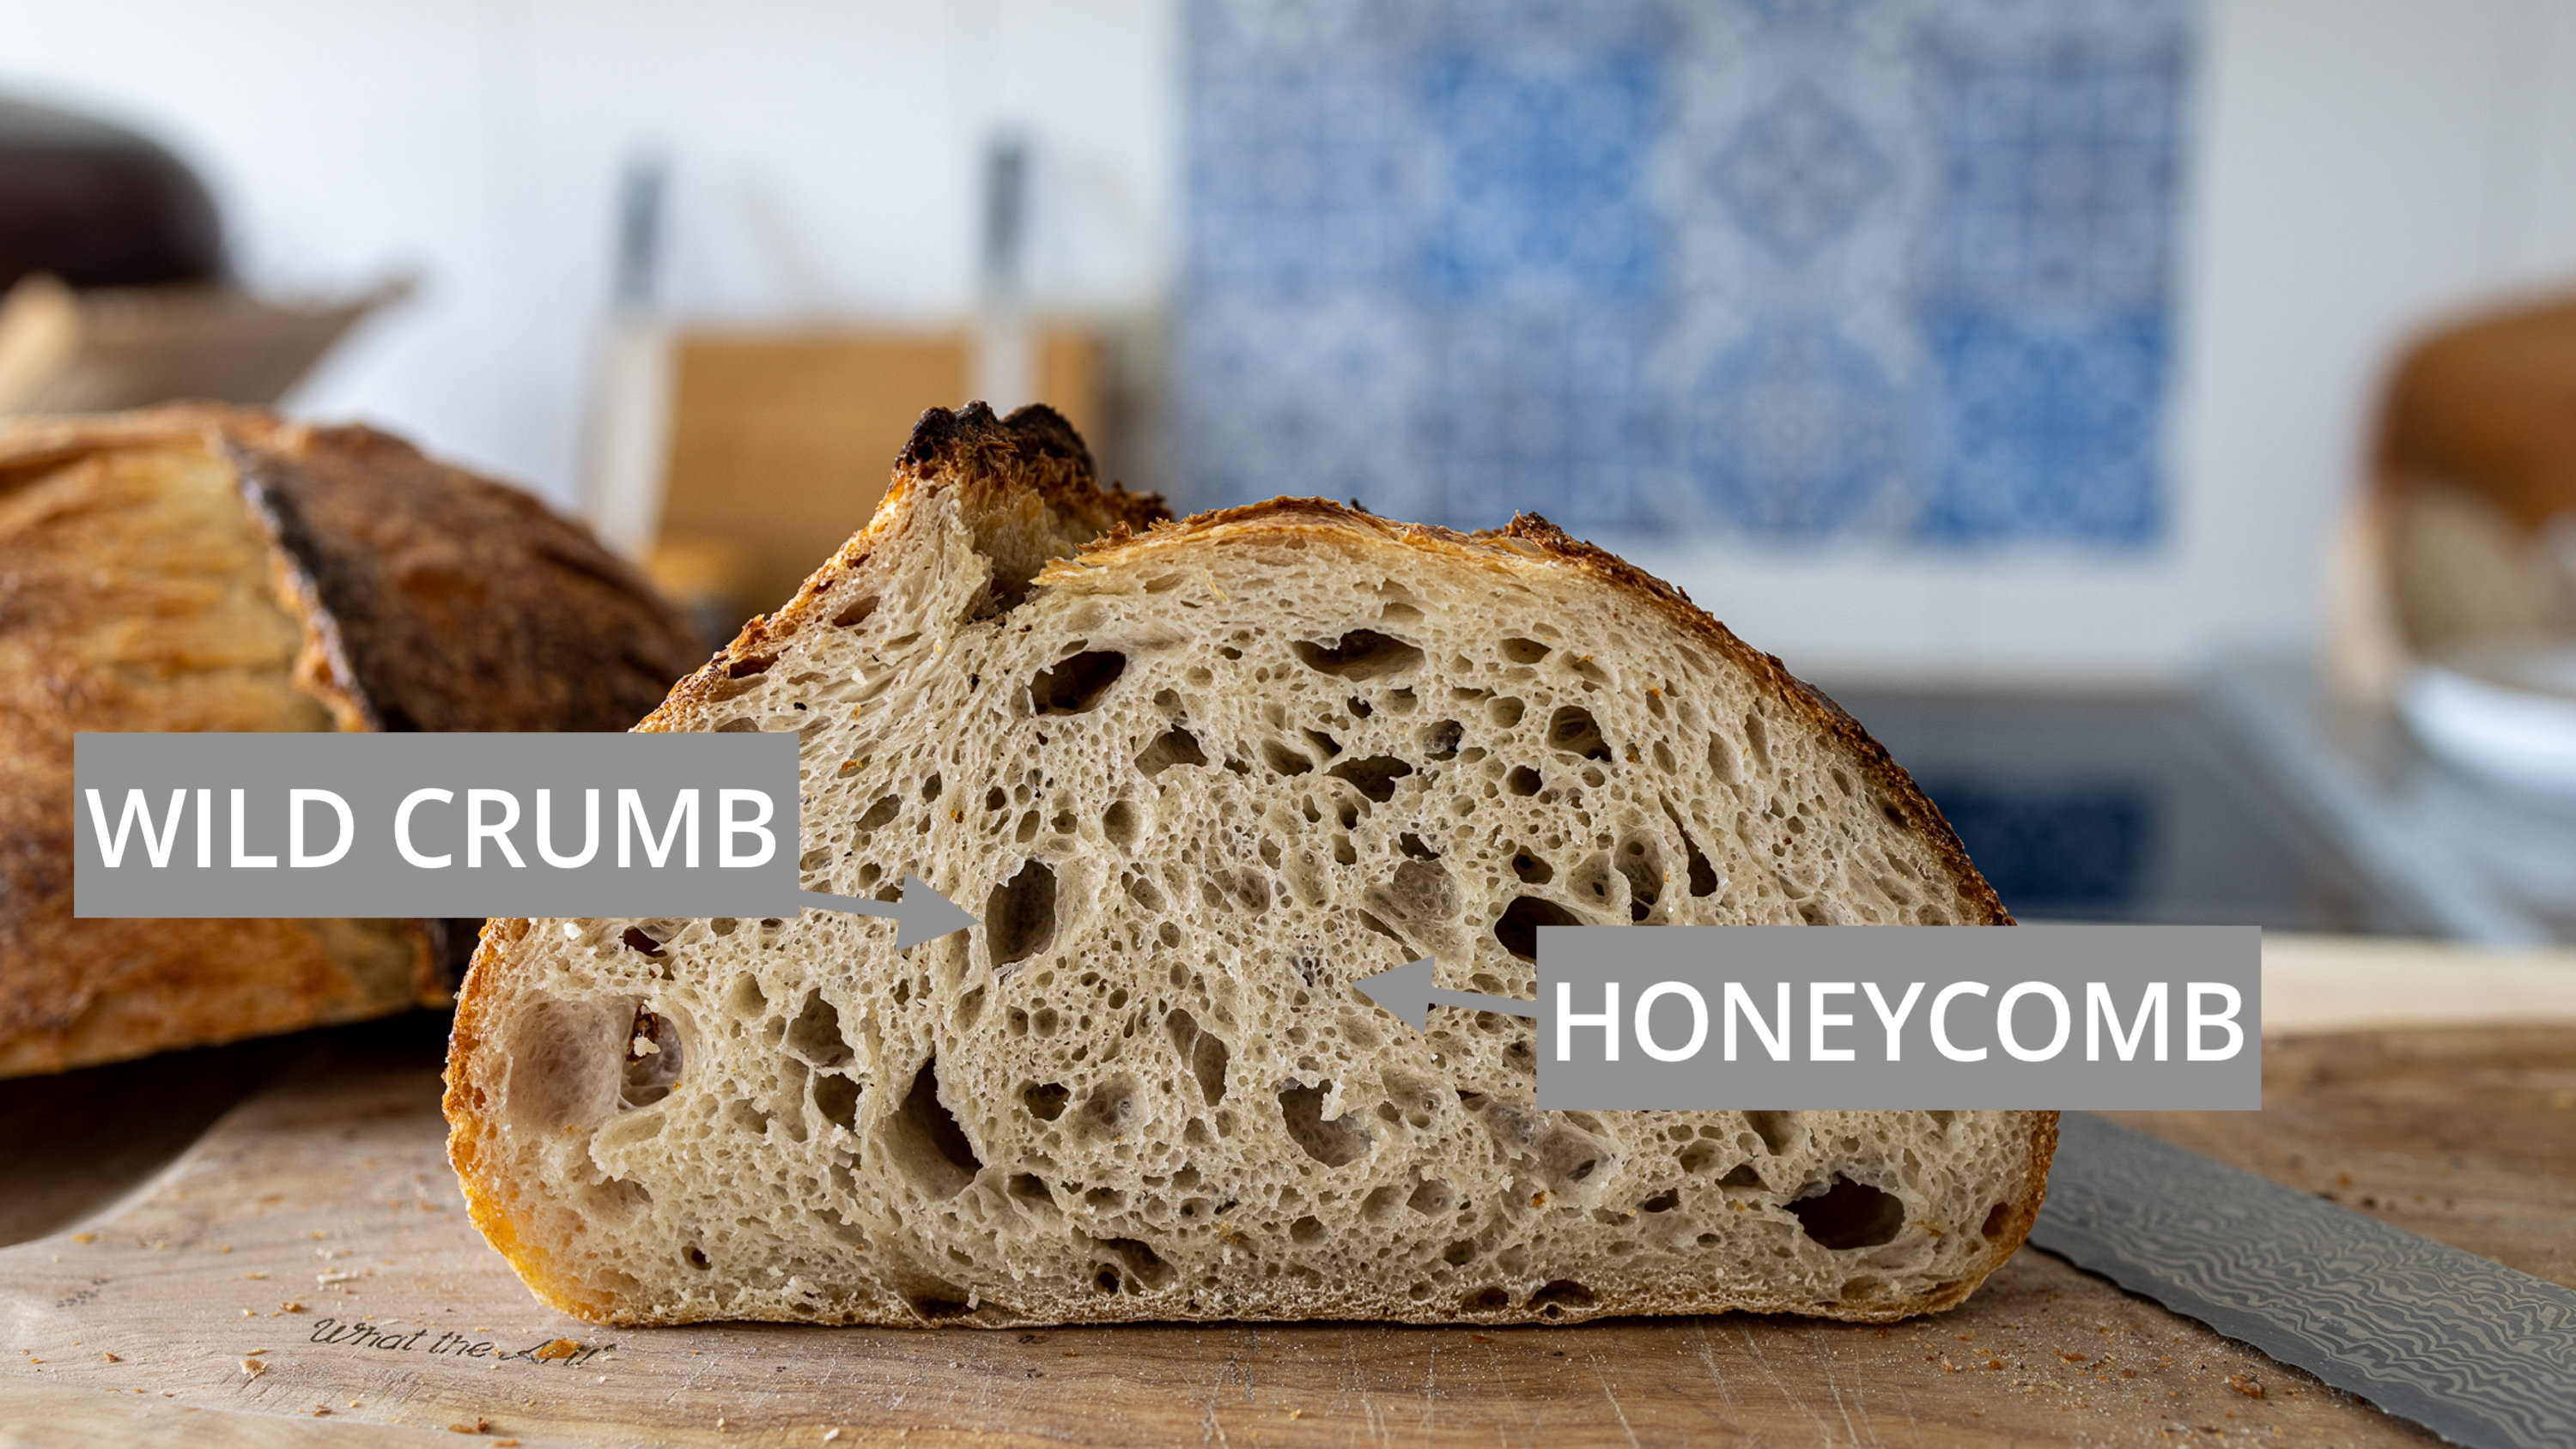
\includegraphics[width=\textwidth]{open-crumb}
  \caption{The bread has a somewhat open crumb with areas
  featuring a honeycomb structure.}
  \label{fig:open-crumb}
\end{figure}

Of course the perfect fermentation is debatable and highly subjective. To
me the perfect sourdough bread features a crisp crust paired with a fluffy
somewhat open crumb. This is the perfect balance of different consistencies
when you take a bite.

Some people are chasers of a very open crumb, meaning you have large pockets
of air (alveoli). It's subjective whether that's the style of bread that you like,
however to achieve it you need to ferment your bread dough perfectly on point.
It takes a lot of skill both in terms of mastering fermentation and technique
to achieve a crumb structure like that.

Me personally I like a bread like that, just with a slightly less wild crumb.
The style of crumb I like is called the {\it honeycomb crumb}. It's not too open, but
just enough open to make the bread very fluffy. To achieve the previously mentioned open crumb you
have to touch your dough as little as possible. The more you interact with your
dough the more you are degassing your dough. Excess touching of the dough
results in the dough's alveoli merging together. The crumb will not be as open.
That's why achieving such a crumb works best if you only ferment
one dough at the same time. Normally if you have to preshape your dough,
you will automatically degas your dough a little bit during the rounding process.
If you skip this step and directly shape your dough you will achieve a more open crumb.
A good rule of thumb is to not touch your dough for at least 1-2 hours before shaping,
to achieve an as open crumb as possible.

\begin{figure}
  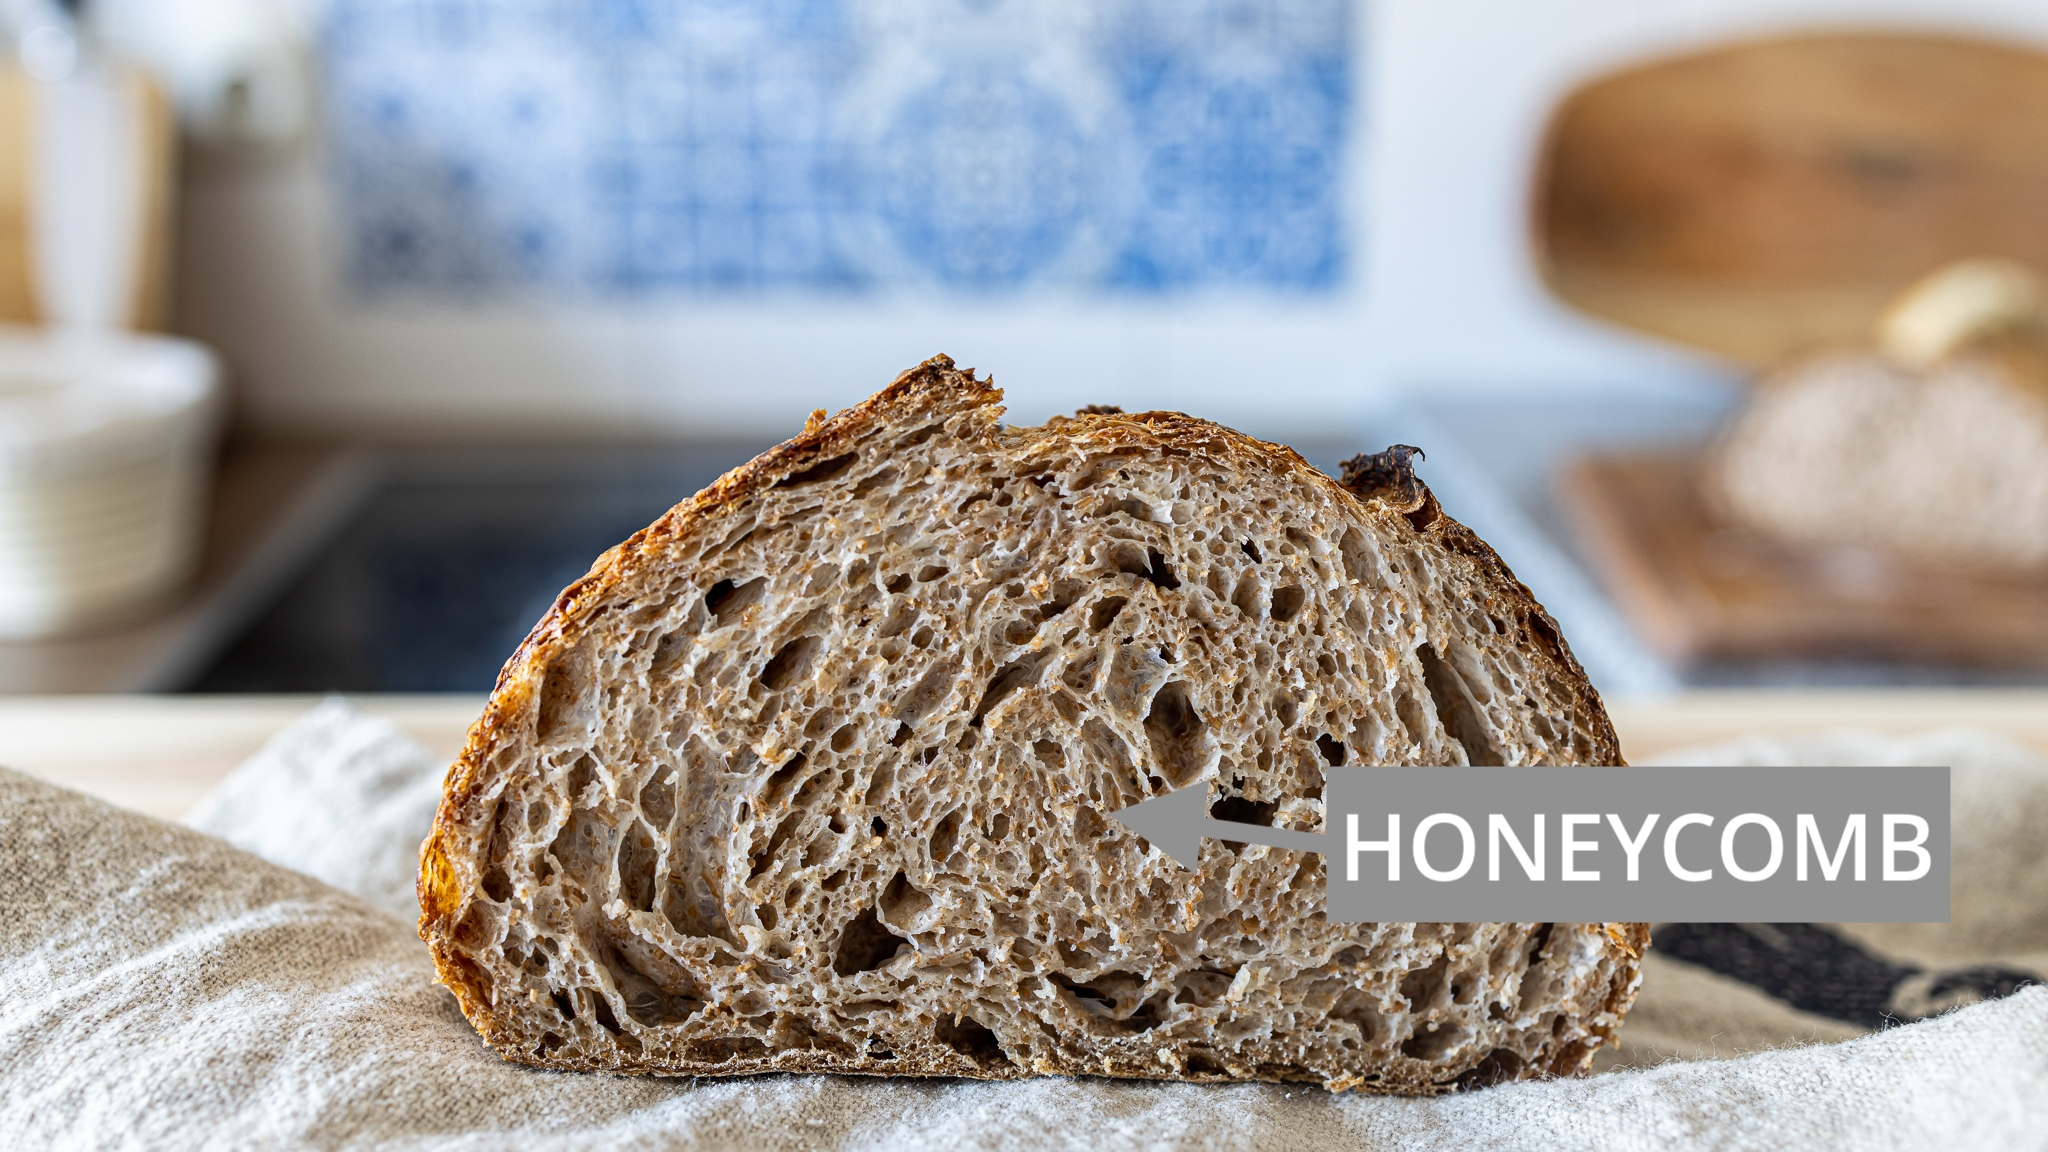
\includegraphics[width=\textwidth]{honeycomb}
  \caption{A whole wheat sourdough with an almost exclusive honeycomb crumb structure.}
  \label{fig:honeycomb}
\end{figure}


Now this is problematic when you want to
make multiple breads at the same time. Preshaping is essential as you are required
to divide your large bulk dough into smaller chunks. Without the preshaping
process you would end up with many non-uniform bread doughs. This technique is
also used when making ciabattas. They are typically not shaped. You only cut the
bulk dough into smaller pieces, trying to work the dough as little as possible.
With preshaping you will converge your dough's alveoli into more of a honeycomb structure,
as large pockets of air will slightly converge. Similarly to the open crumb structure
you also have to nail the fermentation process perfectly to achieve this crumb.
A too long fermentation will result in gas leaking out of your dough while baking.
The honeycomb's won't be able to retain the gas. If you ferment for too short,
there is not enough gas to inflate the structures. To me this is the perfect
style of crumb. As someone who appreciates jam, no jam will fall through a slice
of this bread compared to an open crumb.

\subsection{Overfermented}

\begin{figure}
  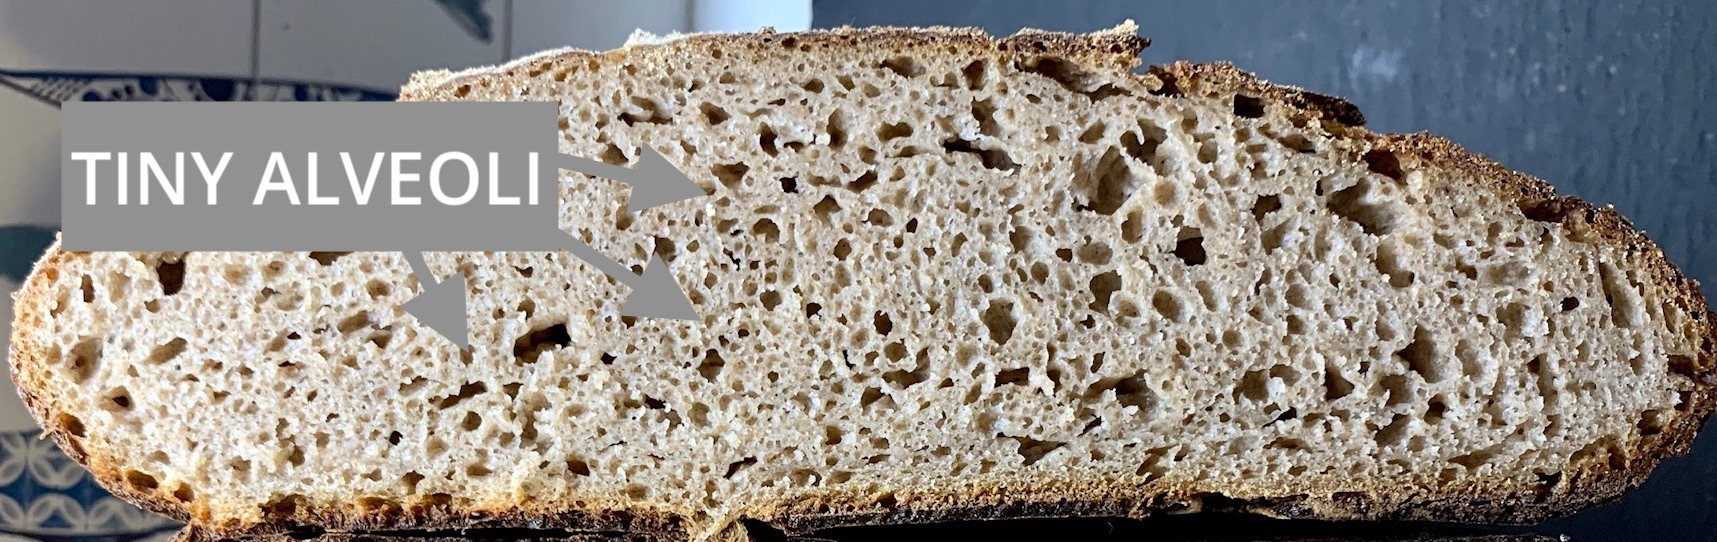
\includegraphics[width=\textwidth]{fermented-too-long}
  \caption{A relatively flat dough that has many tiny pockets of air.}
  \label{fig:fermented-too-long}
\end{figure}

When fermenting your dough for too long over time the protease enzyme starts to
break down the gluten of your flour. Furthermore the bacteria consumes the gluten
in a process called {\it proteolysis} \cite{raffaella+di+cagno}.
Bakers also refer to this process as {\it gluten rot}.
The gluten that normally is normally trapping the CO2 created
by the fermentation process of your microorganisms can no longer stay inside of
the dough. It disperses outward resulting in smaller alveoli in your crumb.
The bread itself tends to be very flat in the oven. Bakers often refer
to this style of bread as a {\it pancake}. The oven spring can be compared
to bread doughs made out of low gluten flour like Einkorn.

Your bread will feature a lot of acidity, a really strong distinctive tang. From
a taste perspective it might be a little bit too sour. From my own tests with family and
friends (n=15-20) I can say that this style of bread is typically
not as appreciated. However, me personally I really like the hearty strong taste.
It is excellent in combination with something
sweet or a soup.  From a consistency perspective it is no longer as fluffy as it could be.
The crumb might also taste a little bit gummy. That's because it has been broken down a lot
by the bacteria. Furthermore this style of bread has a significantly lower amount of gluten \cite{raffaella+di+cagno}
and is no longer comparable to raw flour, it's a fully fermented product.
You can compare it with a blue cheese that is almost lactose free.

When trying to work with the dough you will notice that suddenly the dough feels
very sticky. You can no longer properly shape and work the dough. When trying to
remove the dough from a banneton the dough flattens out very much. Furthermore
in many cases your dough might stick to the banneton. When beginning with baking
I would use a lot of rice flour in my banneton to dry out the surface of the dough a lot.
This way the dough wouldn't stick, despite being over fermented. However as it
turns out the stickiness issue has been my lack of understanding the fermentation
process. Now I never use rice-flour, except when trying to apply decorative scorings.
Properly managing fermentation results in a dough that is not sticky.

If you are noticing during a stretch and fold, or during shaping that your dough
is suddenly overly sticky, then the best option is to use a loaf pan. Simply take
your dough and toss it into a loaf pan. Wait until the dough mixture has increased
in size a bit again and then bake it. You will have a very well tasting sourdough
bread. If it's a bit too sour, you can just bake your dough for a longer period
of time to boil some of the acidity during the baking process. You can also use
your dough to setup a new starter and try again tomorrow. Lastly if you are hungry
you can simply pour some of your dough directly into a heated pan with a bit of
oil. You will be making delicious sourdough flat breads.

To fix issues related to overfermentation you need to stop the fermentation process
earlier. What I like to do is to extract a small fermentation probe from my dough.
Depending on the volume increase of this probe I can mostly judge when my fermentation
is finished. Try to start with a 25 percent volume increase of your main dough or sample.
Depending on how much gluten your flour has, you can ferment for a longer period of time.
With a strong flour featuring a 14-15 percent protein you should be able to safely
ferment until a 100 percent size increase. This however also happens on your
sourdough starter's composition of yeast and bacteria. The more bacterial fermentation
the faster your dough structure breaks down. Frequent feedings of your sourdough
starter will improve the yeast activity. Furthermore a stiff sourdough starter
might be a good solution too. The enhanced yeast activity will result in a more fluffy
dough with less bacterial activity. A better yeast activity also will result
in less acidity in your final bread. If you are a chaser of a very strong tangy
flavor profile then a stronger flour with more gluten will help.


\subsection{Underfermented}

\begin{figure}
  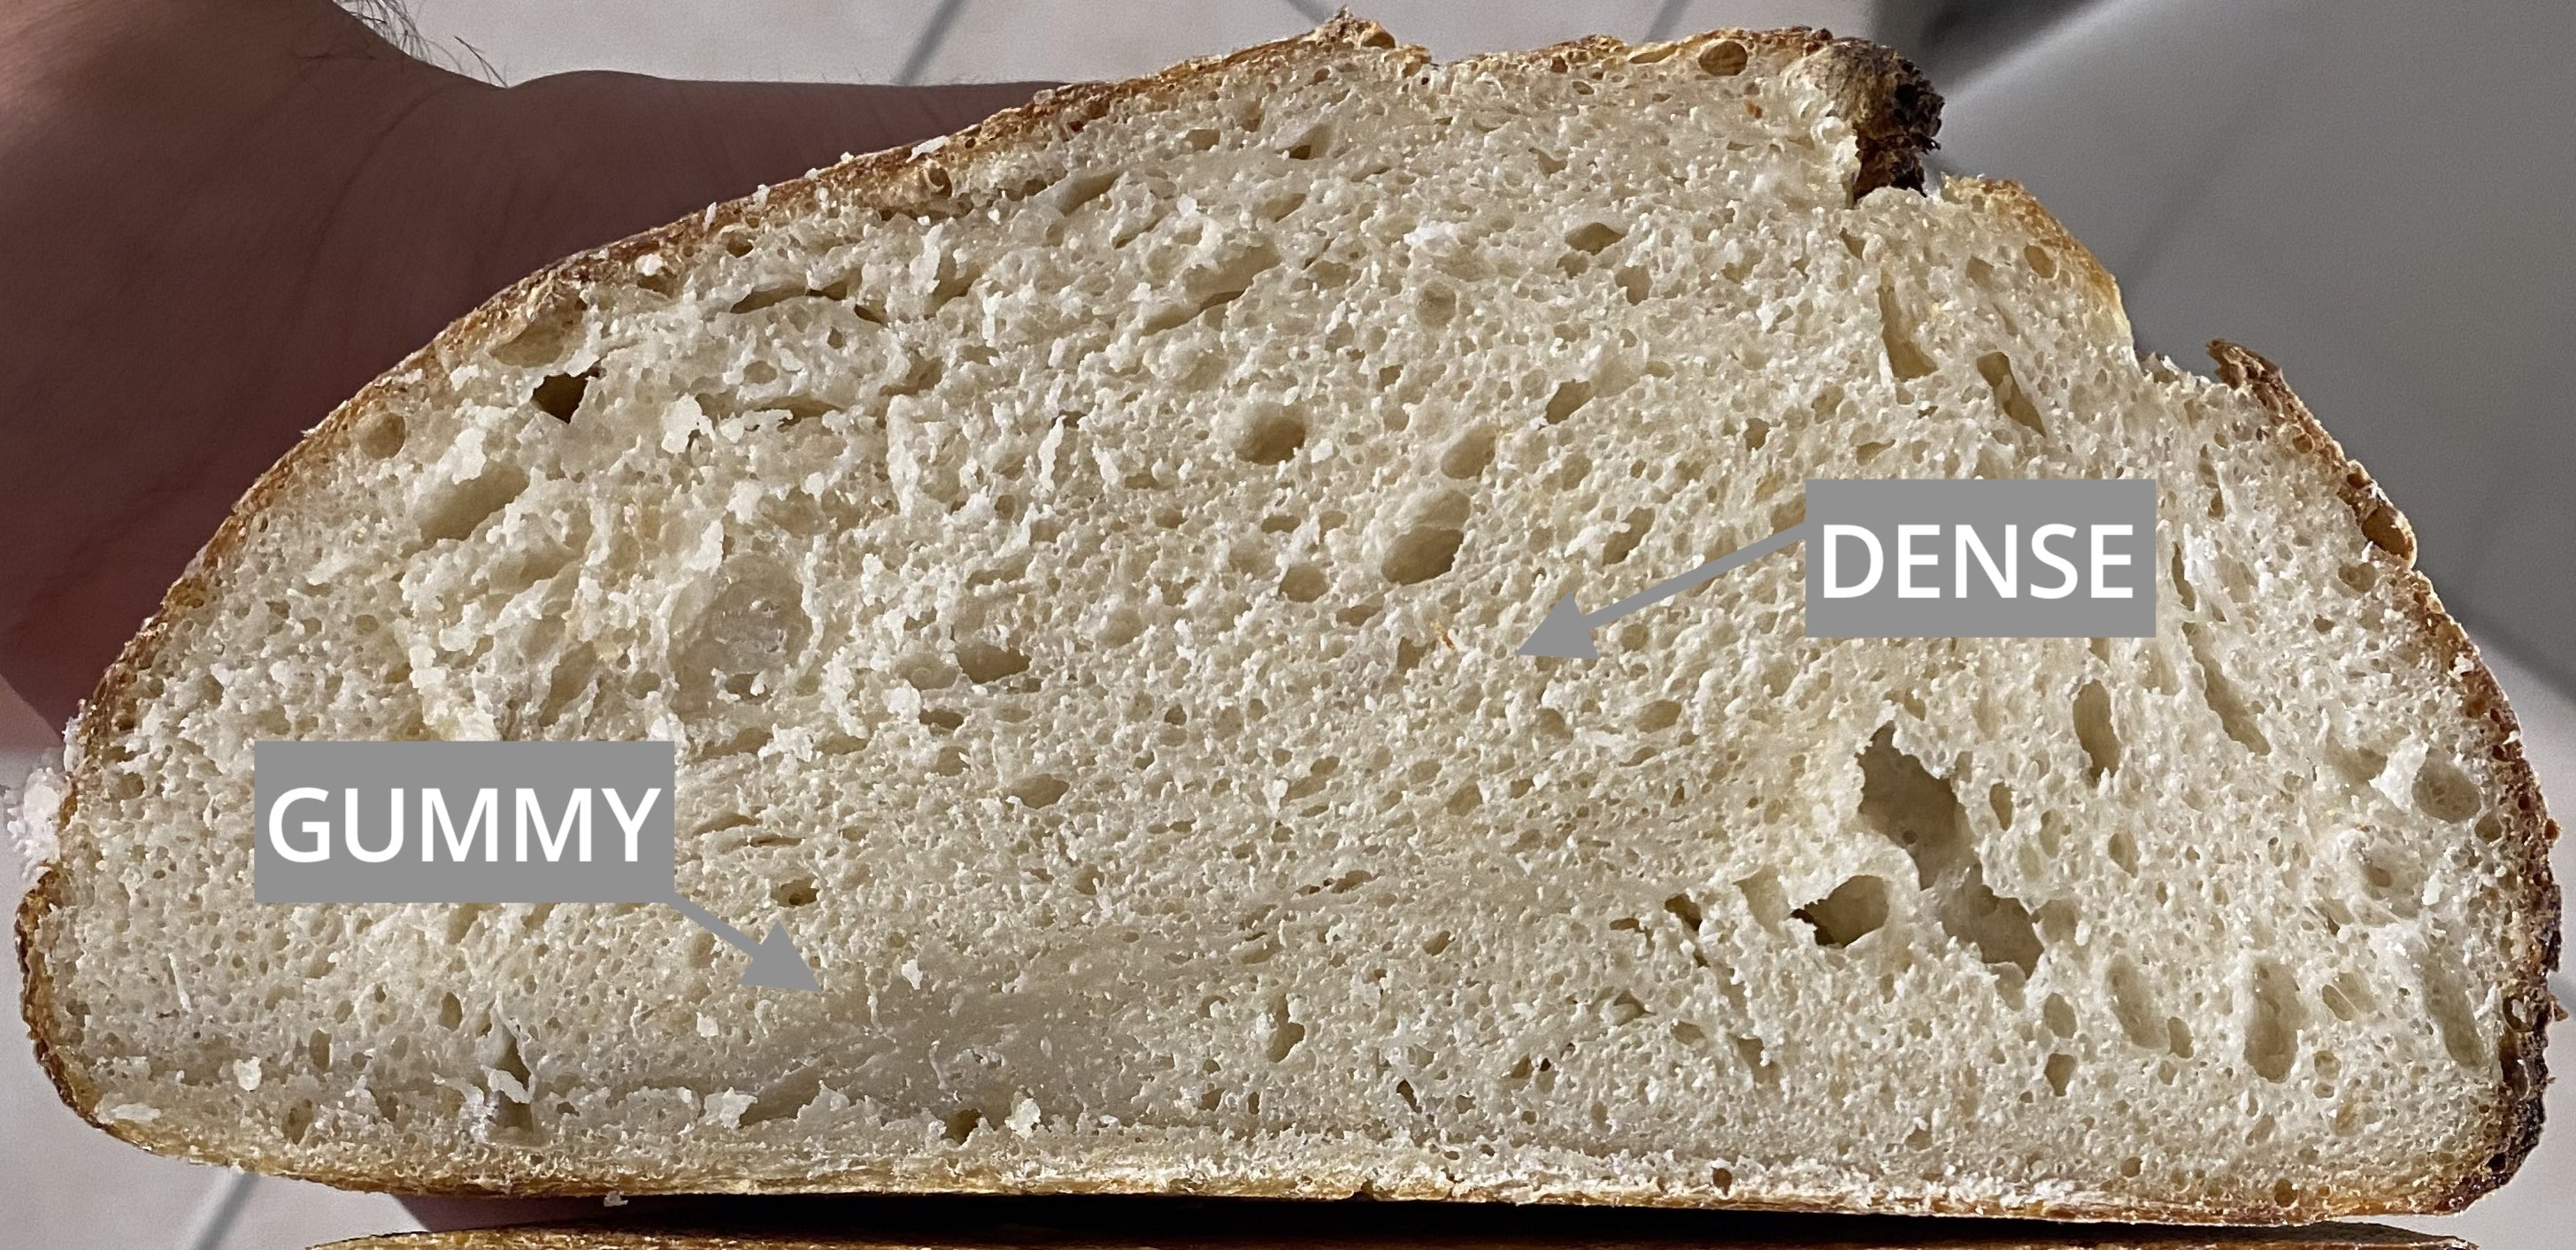
\includegraphics[width=\textwidth]{fermented-too-short-underbaked}
  \caption{A dense dough featuring a gummy not fully gelatinized area.
  The picture has been provided by Midori from our community discord server.}
  \label{fig:fermented-too-short-underbaked}
\end{figure}

This defect is also commonly referred to as {\it underproofed}. However underproofed
is not a good term as it only refers to having a too short period of time in the final
proofing stage of the bread making process. If you were to directly bake your bread
after a successful bulk fermentation stage you would not achieve this defect.
Proofing will make your dough a bit more extensible and allows your sourdough
to inflate the dough a bit more. When faced with an underfermented bread you
already did something wrong during the bulk fermentation stage, or maybe also
even before that with your sourdough starter.

A typical underfermented dough has very large pockets of air and is partially
wet and gummy in some areas of the dough. The large pockets can be compared
to making a non-leavened wheat or corn tortilla. As you bake the dough in your pan
the water slowly starts to evaporate. The gas is trapped in the structure of the dough
and will create pockets. In case of a tortilla this is the desired behavior.
But when you observe this process in a larger dough you will create several
super alveoli. The water evaporates and the first alveoli form. Then at some point
the starch starts to gelatinize and becomes solid. This happens first inside of the pockets
as the interior heats up faster compared to the rest of the dough. Once all the starch
has gelatinized the alveoli holds its shape and no longer expands. During this
process other parts of the bread dough are pushed outwards. That's why an underfermented
dough sometimes even features an ear during the baking process. This
is also commonly referred to as a {\it fool's crumb}. You are excited about an ear which
can be quite hard to achieve. Plus you might think you finally created some big pockets
of air in your crumb. But in reality you fermented for a too short period
of time.

\begin{figure}
  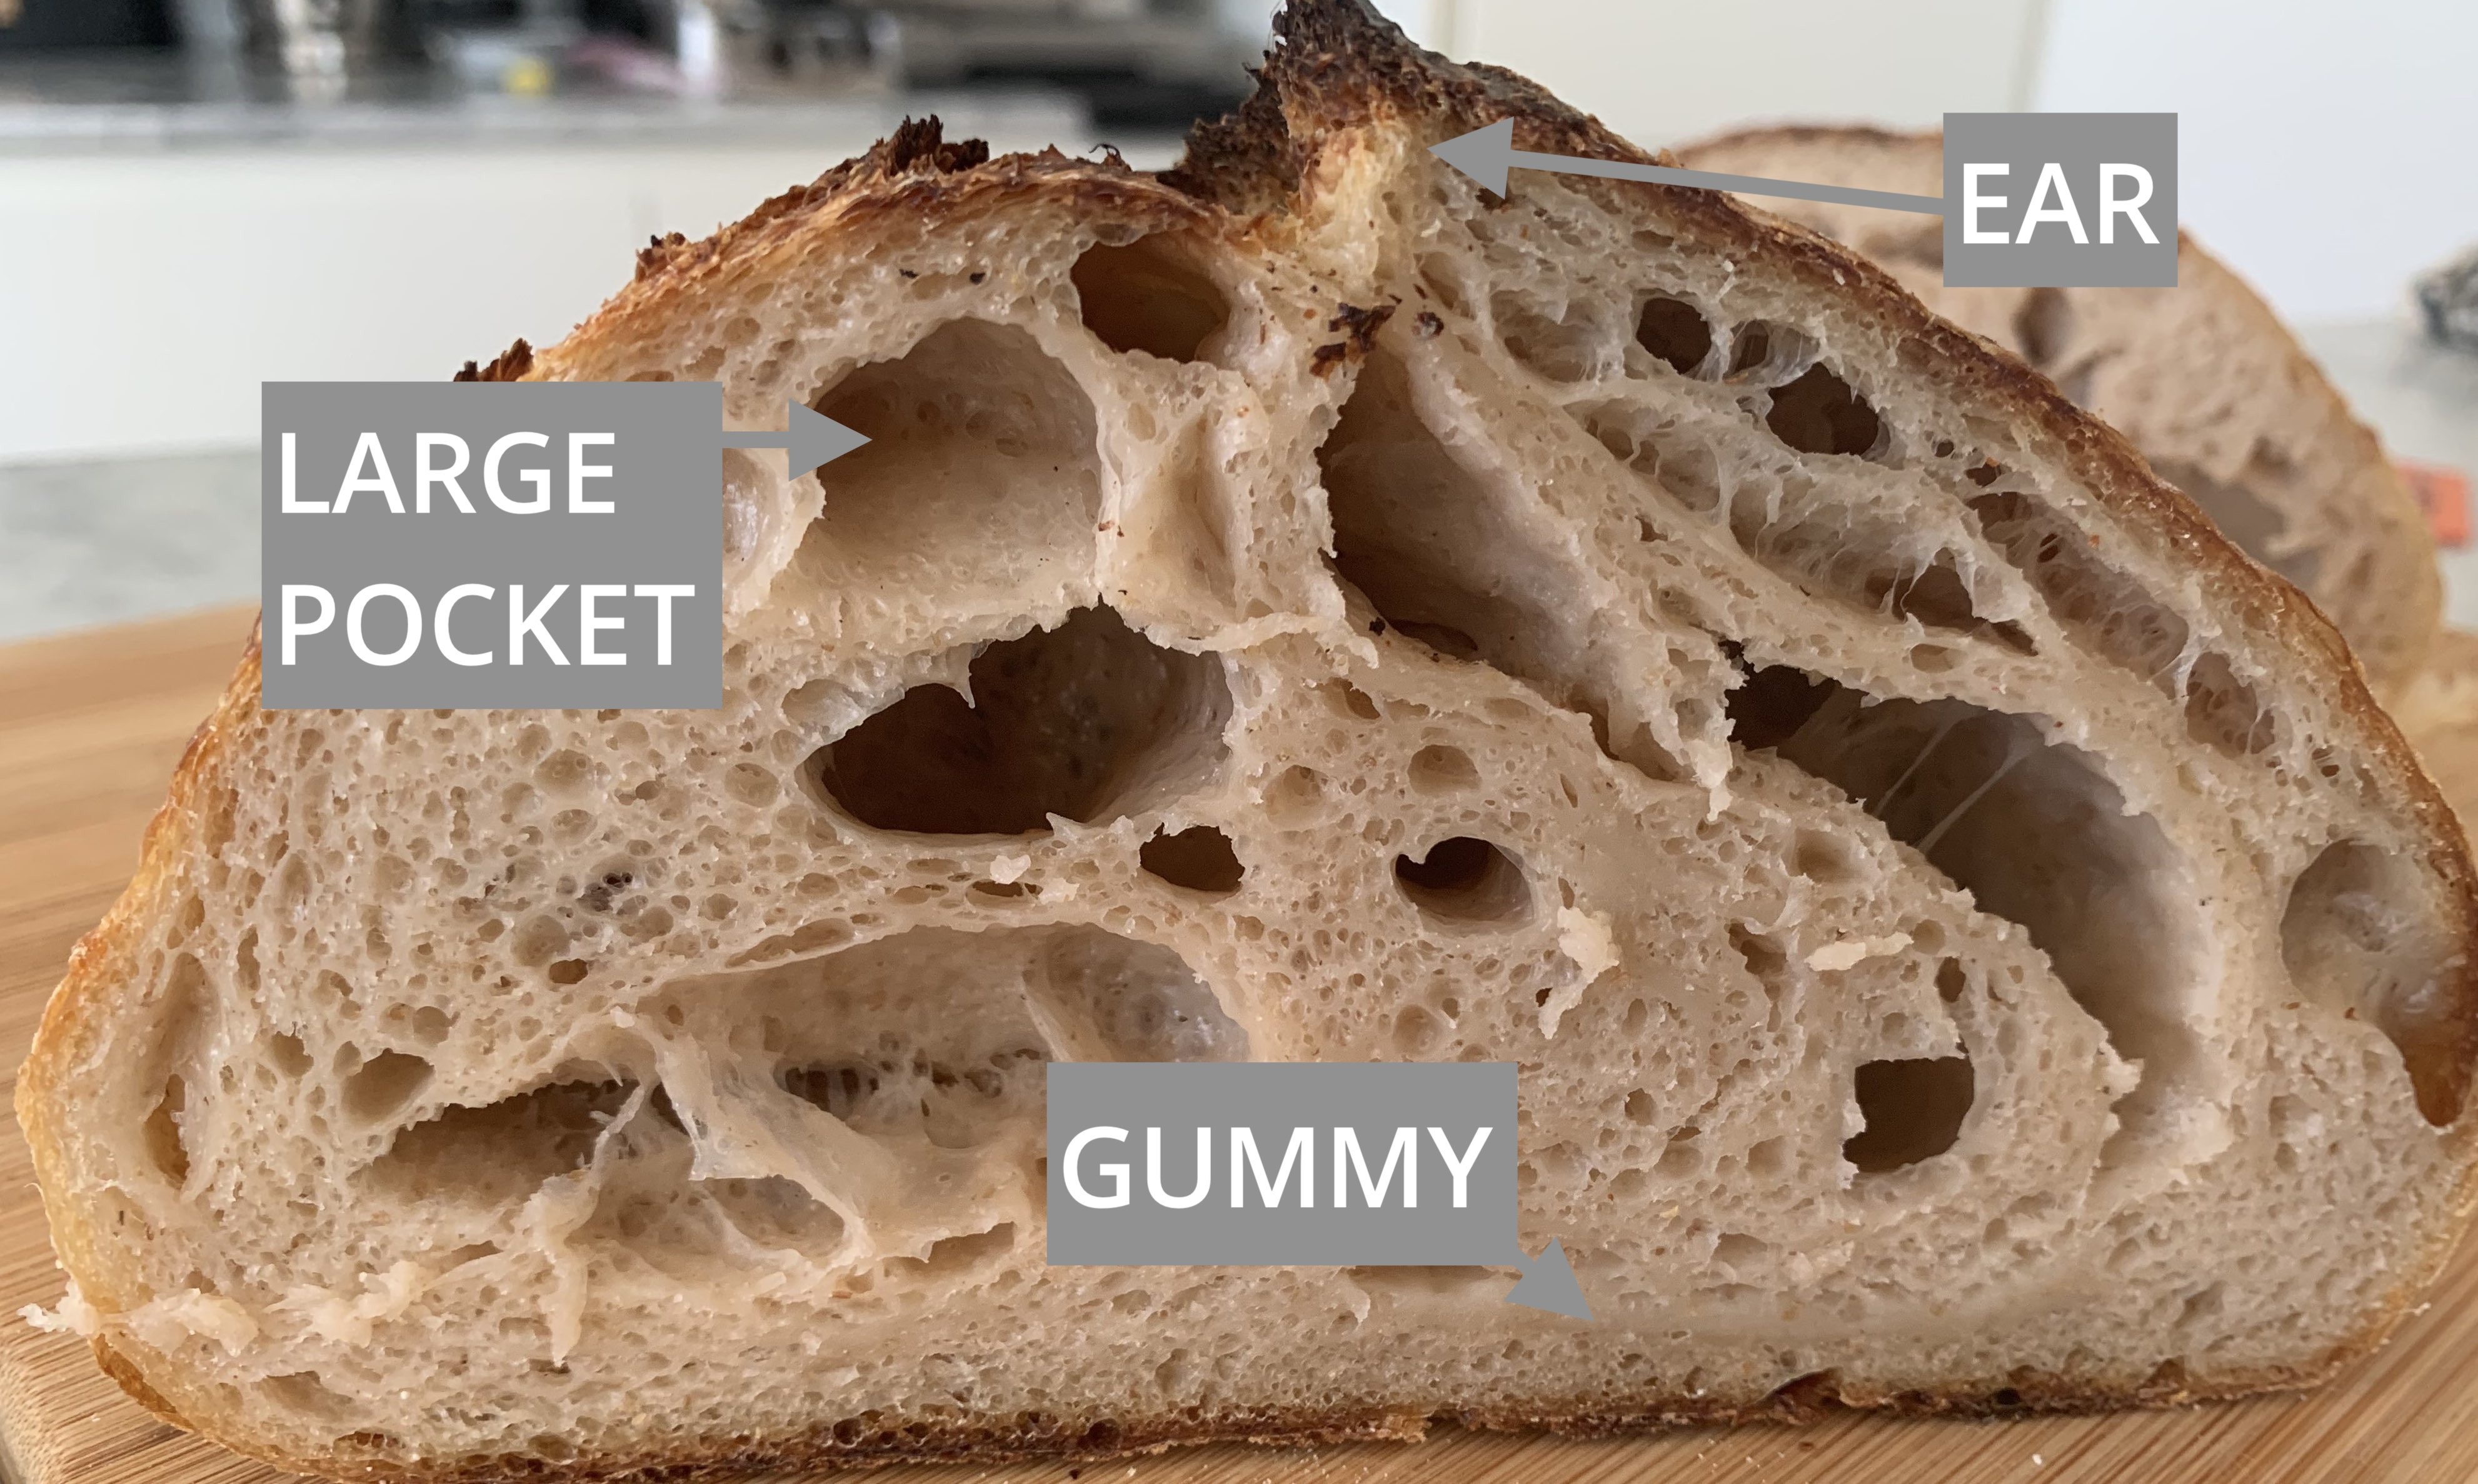
\includegraphics[width=\textwidth]{fools-crumb}
  \caption{A typical example of a fool's crumb featuring an ear and several overly
  large alveoli. The picture has been provided by Rochelle from our
  community discord server.}
  \label{fools-crumb}
\end{figure}

In a properly fermented dough the alveoli help with the heat transfer throughout the dough.
From within the tiny many fermentation induced pockets the starch gelatinizes. With
an underfermented dough this heat transfer does not properly work. Because of that
you sometimes have areas which look like raw dough. Bakers refer to this as a very
gummy structure sometimes. Baking your dough for a longer period of time would also properly
gelatinize the starch in these areas. However, then other parts of your bread
might be baked too long.

To fix issues related to underfermentation you simply have to ferment your dough
for a longer period of time. Now there is an upper limit to fermentation time
as your flour breaks down the moment it is in contact with water. That's why it
might be a good idea to simply speed up your fermentation process. As a rough
figure, I try to aim for a bulk fermentation time of around 8-12 hours typically.
To achieve that you can try to make your sourdough starter more active.  This can be done
by feeding your starter daily over several days. Use the same ratio as you would
do for your main bread dough. Assuming you use 20 percent starter calculated on the flour,
use a 1:5:5 ratio to feed your starter. That would be 10 grams of existing starter,
50 grams of flour, 50 grams of water for instance. To boost your yeast even more you can
consider making a stiff sourdough starter. The stiff sourdough starter will
boost your yeast activity. The bacteria produces mostly acid. The more acidity
is piled up, the less active your yeast is. The stiff sourdough starter
enables you to start your dough's fermentation with yeast dominated activity.


\subsection{Not enough dough strength}

\begin{figure}
  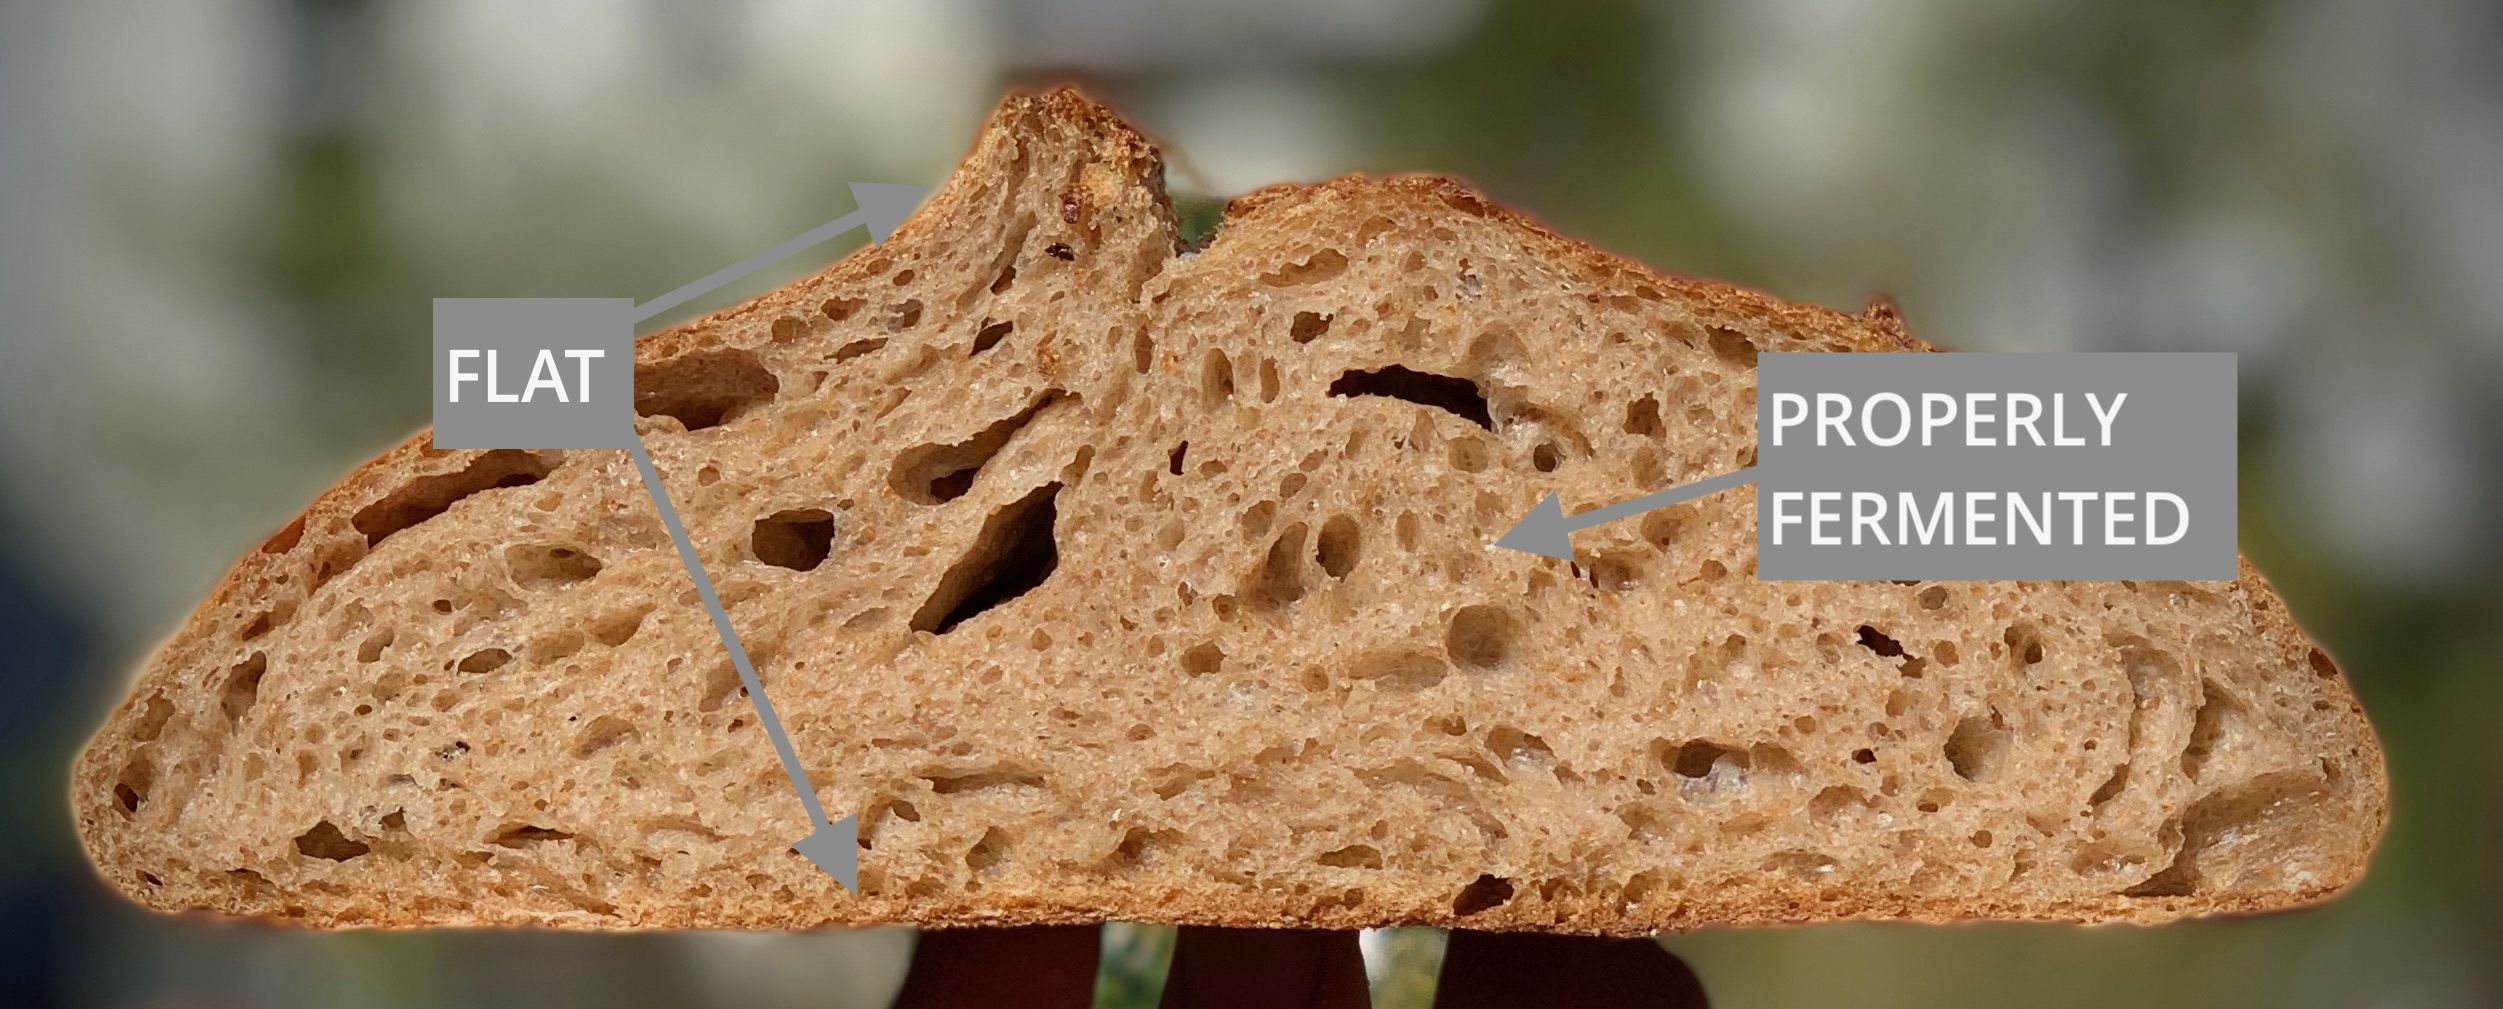
\includegraphics[width=\textwidth]{flat-bread}
  \caption{A very flat bread without enough dough strength.}
  \label{flat-bread}
\end{figure}

When a dough flattens out quite a lot during the baking process chances are
that you did not create enough dough strength. This means your gluten matrix
hasn't been developed properly. Your dough is too extensible and flattens out
mostly rather than springing upwards in the oven. This can also happen if you
proofed your dough for too long. Over time the gluten relaxes and your dough
becomes more and more extensible. You can observe the gluten relaxing behavior
too when making a pizza pie. Directly after shaping your dough balls it's very hard to shape
the pizza pie. If you wait for 30-90 minutes stretching the dough becomes a lot easier.

The easiest way to fix this is probably to knead your dough more at the start. To simplify
things consider using less water for your flour too. This will result in a more elastic dough
right away. This concept is commonly used for no-knead style sourdough.  Alternatively you
can also perform more stretch and folds during the bulk fermentation process. Each
stretch and fold will help to strengthen the gluten matrix and make a more elastic dough.
The last option to fix a dough with too little dough strength is to shape your dough tighter.

\subsection{Baked too hot}

\begin{figure}
  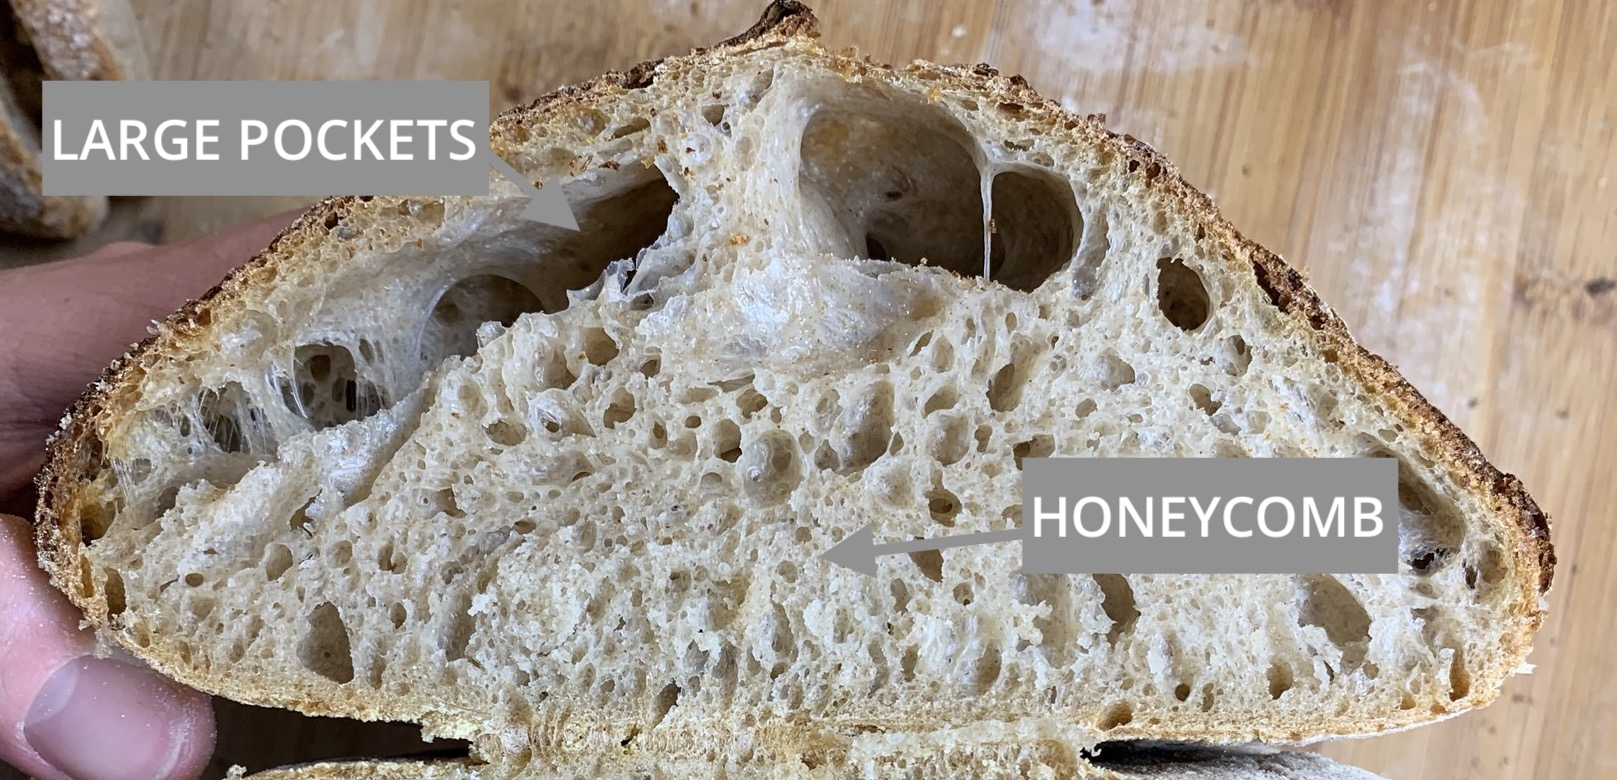
\includegraphics[width=\textwidth]{baked-too-hot-v2}
  \caption{A bread with very large alveoli close to the crust}
  \label{baked-too-hot}
\end{figure}

This is a common mistake that has happened to me a lot. When you bake your dough
at a too hot temperature you block your dough's expansion. The starch gelatinizes
and becomes more and more solid. At around 140°C (284°F) the maillard reaction
starts to completely thicken your bread dough's crust. This is similar to baking
your bread dough without steam. As the internal dough's temperature heats up
more and more water evaporates, gas expands and the dough is being pushed upwards.
Once the dough reaches the crust it can no longer expand. The alveoli merge
into larger structures close to the surface of the dough. By baking too hot
you are not achieving the ear which adds extra flavor. Furthermore your crumb
is not as fluffy as it could be by restricting its expansion capabilities.

If you have an extensible dough with high hydration baking too cold will result
in the dough flattening out quite a lot. The gelatinization of the starch is
essential for the dough to hold it's structure. After conducting several
experiments it seems that my sweet spot for maximum oven spring seems to be
at around 230°C (446°F). Test the temperature of your oven, because in several
cases the displayed temperature might not match the actual temperature of your
oven \cite{too+hot+baking}. Make sure to turn off the fan of your oven. Most
home ovens are designed to vent the steam as fast as possible. If you can not
turn the fan off, consider using a dutch oven.

\subsection{Baked with too little steam}

\begin{figure}[h]
  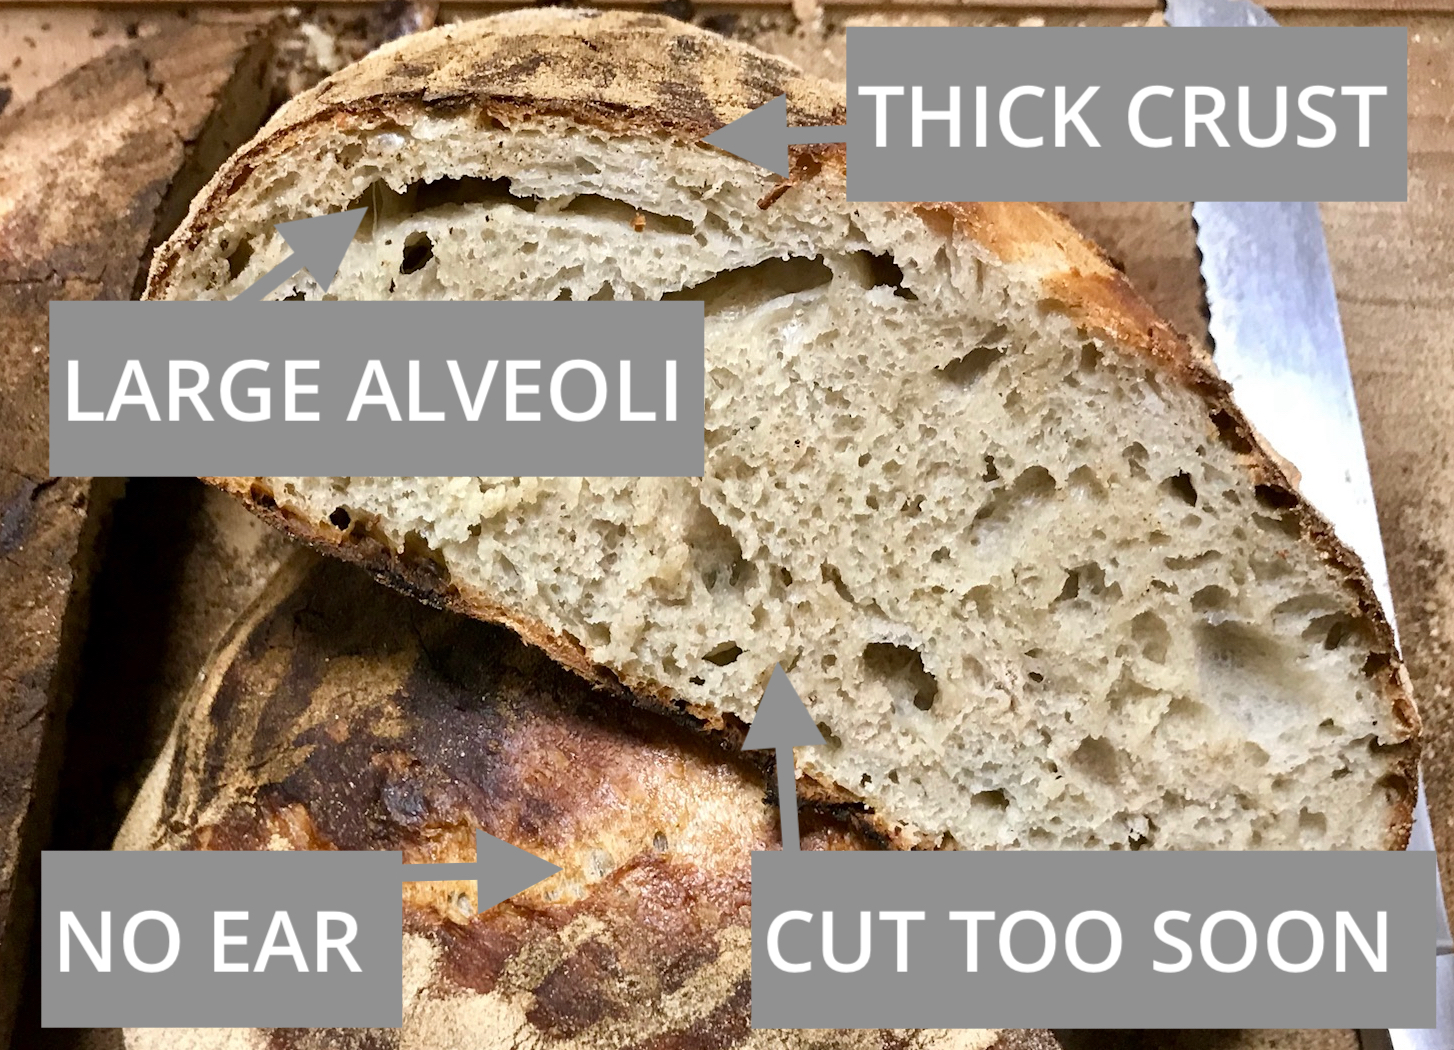
\includegraphics[width=\textwidth]{no-steam}
  \caption{One of my earlier breads that I baked at a friend's place where
  I couldn't steam the dough properly}
  \label{no-steam}
\end{figure}

Similarly to baking too hot when baking without enough steam your dough's crust
forms too quickly. It's hard to spot the difference between the two mistakes.
I typically first ask about the temperature and then about the steaming technique
to determine what might be wrong with the baking process. Too little steam can
typically be spotted by having a thick crust around all around your dough paired
with large alveoli towards the edges.

The steam essentially prevents the maillard reaction from happening too quickly
on your crust. That's why steaming during the first stages of the bake is so important.
The steam keeps the temperature of your crust close to around 100°C (212°F). Achieving steam
can be done by using a dutch oven, an inverted tray and or a bowl of boiling water.
You might also have an oven with a built-in steam functionality. All the methods work,
it depends on what you have at hand. My default go-to method is an inverted
tray on top of my dough, paired with a bowl full of boiling water towards the bottom
of the oven.

\begin{figure}
  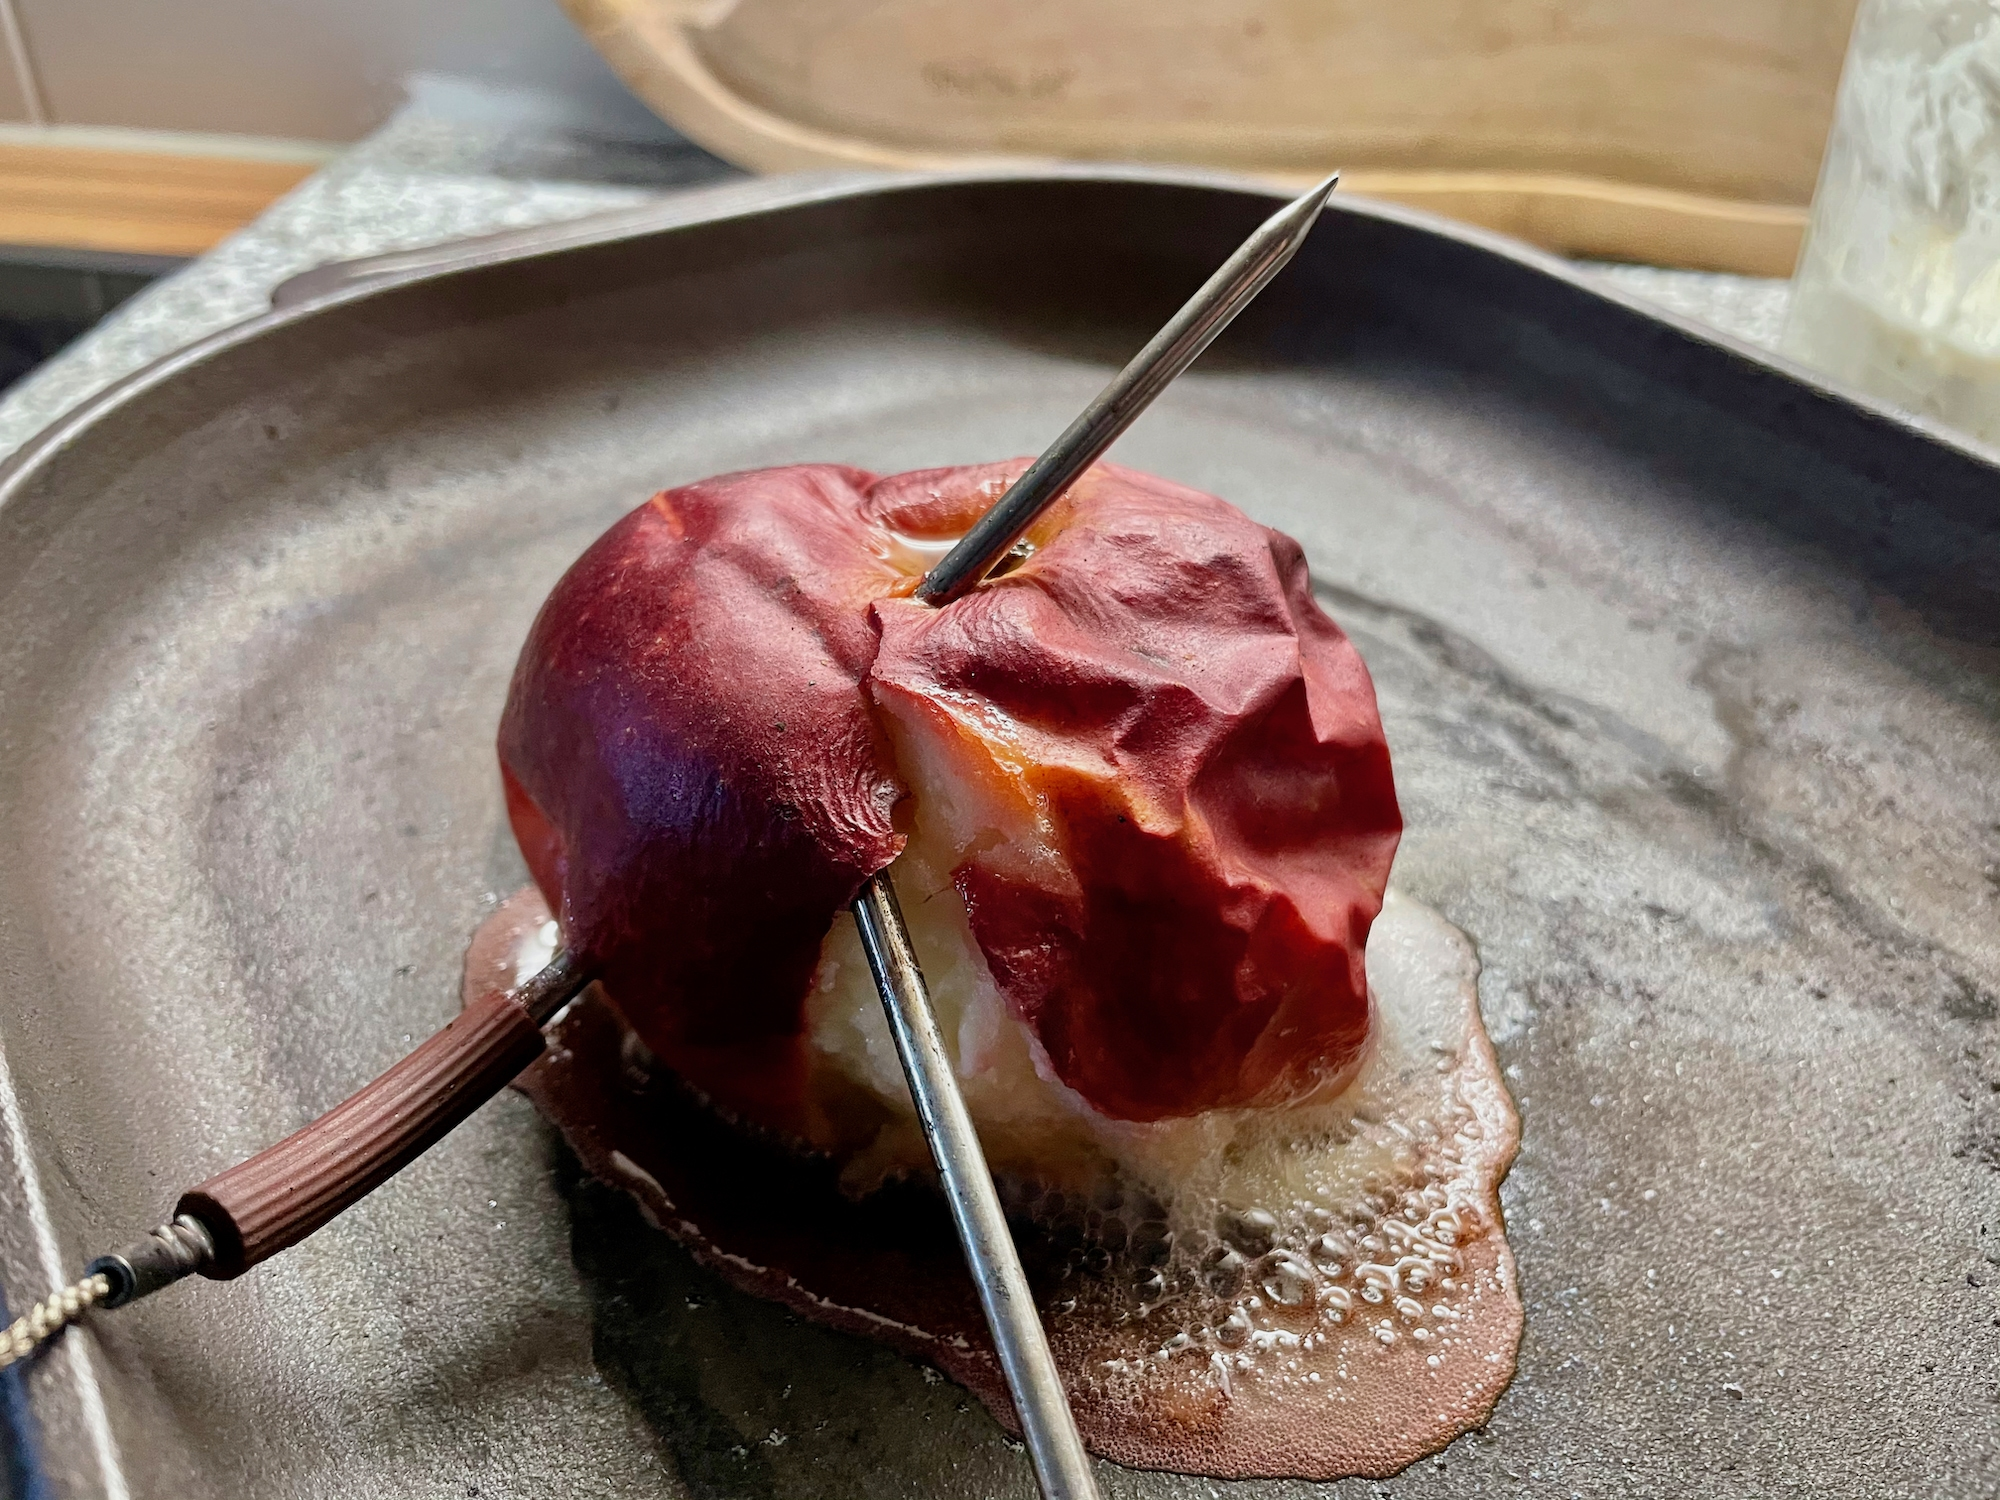
\includegraphics[width=\textwidth]{apple-experiment-temperatures}
  \caption{An apple with 2 probes to measure ambient
  and surface temperatures of several steaming techniques
  in a dutch oven.}
  \label{apple-experiment-temperatures}
\end{figure}

Now there can also be too much steam. For this I tested using a dutch oven paired with large ice
cubes to provide additional steam. The temperature of my dough's surface would directly
jump close to 100°C. The steam contains more energy and can thus through convection
heat up the surface of your dough faster. I tested this by using an apple inside of
a dutch oven. Then I would use a barbecue thermometer with a probe directly at the surface.
I would then change the steaming methods to plot how quickly the temperature
close to the surface of the dough changes. I tried to use an ice cube inside of a preheated
dutch oven, a preheated dutch oven, a preheated dutch oven with spritzes
of water on the apple's surface, a non preheated dutch oven where I would only preheat
the bottom part. The experiment then showed that the ice-cube method would heat up
the surface of the apple a lot quicker. When replicating this with a bread dough
I would achieve less oven spring.

\begin{figure}[h]
  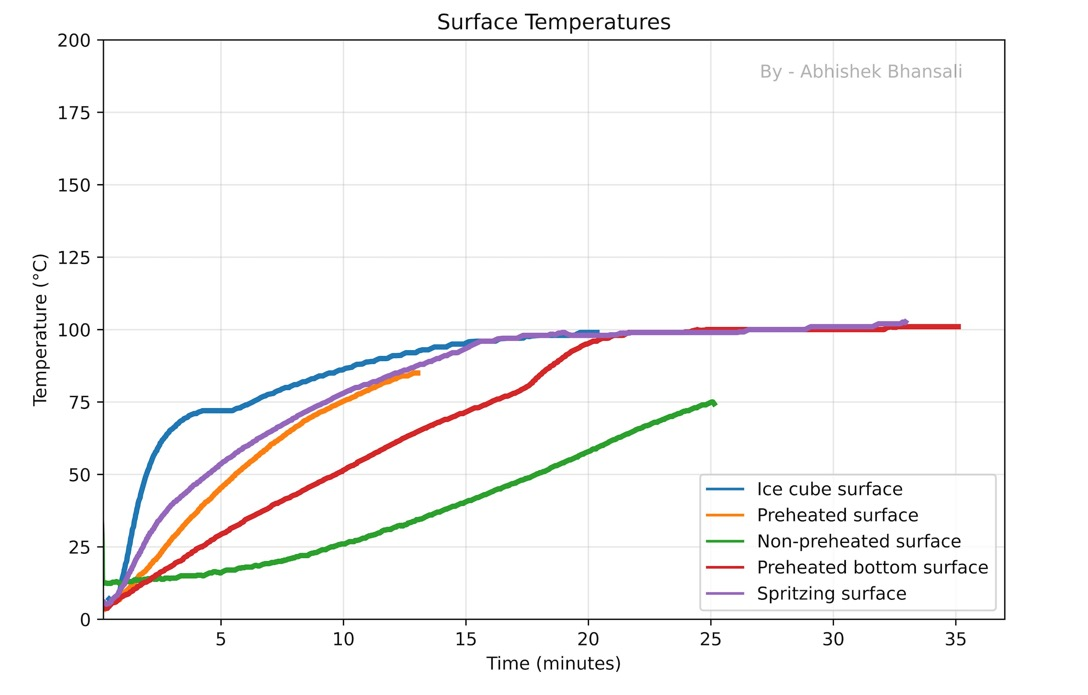
\includegraphics[width=\textwidth]{apple-experiment-surface-temperatures}
  \caption{A chart showing how the temperature of the surface
  of the apple changes with different steaming techniques.}
  \label{apple-experiment-surface-temperatures}
\end{figure}

\begin{figure}[h]
  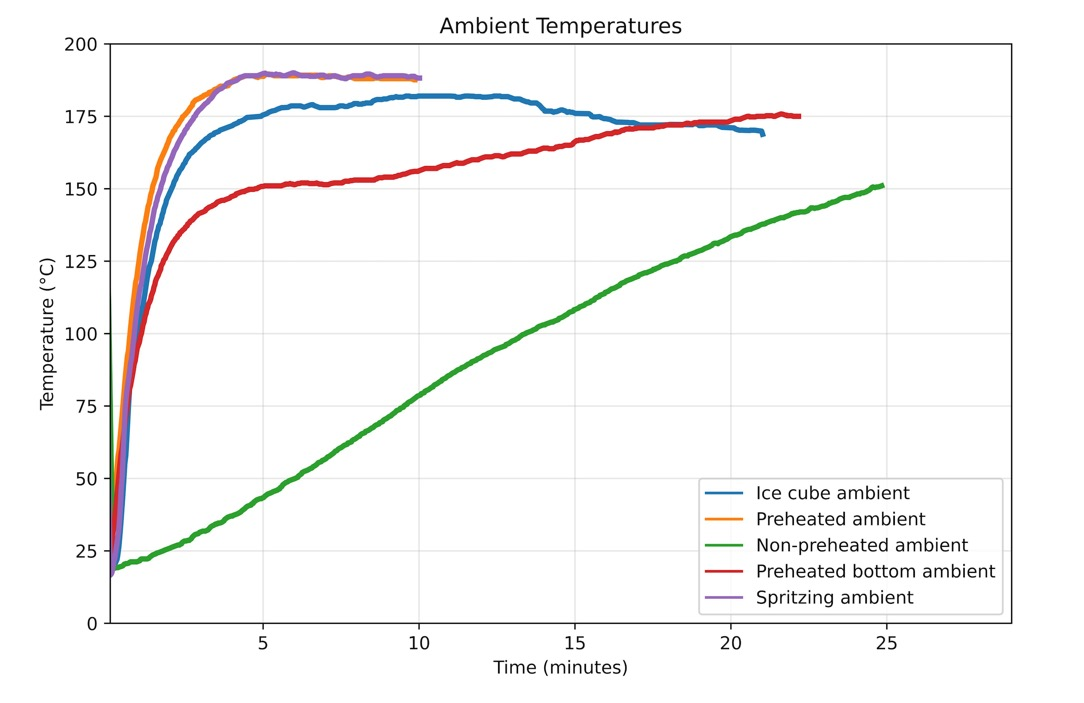
\includegraphics[width=\textwidth]{apple-experiment-ambient-temperatures}
  \caption{This figure shows how the ambient temperatures inside of the
  dutch oven change depending on the steaming technique that is used.}
  \label{apple-experiment-ambient-temperatures}
\end{figure}

Generally though achieving too much steam is relatively challenging. I could only
commit this mistake when using a dutch oven as steaming method paired with relatively
large ice cubes. After talking with other bakers using the same dutch oven, it seems
that mine (around 80g) were 4 times as heavy as the ones other bakers would use (20g)
\section{Baking in the tropics}

Depending on the temperature your fermentation speed adapts.
In a warmer environment everything is faster. In a colder
environment everything is slower.

This includes the speed at which your sourdough ferments
the dough but also the speed of enzymatic reactions. The
amylase and protease enzymes work faster, making more
sugars available and degrading the gluten proteins.

At around 22°C in my kitchen my bulk fermentation is ready
after around 10 hours. I am using around 20 percent of sourdough
starter based on the flour. In summer times the temperatures
in my kitchen sometimes increase to 25°C. In that case
I am reducing the sourdough starter to around 10 percent.
If I wouldn't do that my fermentation would be done after
around 4-7 hours. The problem is that the dough is quite
unstable when fermenting at this high speed. This means
that you are easily running into issues of overfermentation.
Finding the perfect sweet spot between fermenting enough
and not too much is becoming much harder. Normally you might
have a time window of 1 hour. But at the rapid speed it
might be reduced to a time window of 20 minutes. Now at
30°C ambient temperature things are way faster. Your bulk
fermentation might be complete in 2-4 hours when using
10-20 percent starter. Proofing your dough in the fridge
becomes almost impossible. As your dough cools down in the
fridge the fermentation also slows down. However cooling the
dough down from 30°C to 4-6°C in your fridge takes much
longer. Your dough is much more active compared to a dough
that starts at a temperature of 20-25°C. You might
end up overproofing your dough if you leave it overnight
in the fridge.

That's why I recommend that you reduce the amount of starter
that you use in the tropics to something at around 1-5 percent
based on the flour. This will slow down the fermentation
process significantly and provides you a bigger window
of time. Try to aim for an overall bulk fermentation of at
least 8-10 hours. Reduce the amount of starter to get there.

When making a dough try to use the same water temperature
as your ambient temperature. Assuming that the temperature
will climb to 30°C, try to start your dough directly
with 30°C water. This means that you can carefully rely on
a small fermentation probe that visualizes your fermentation
progress. The probe only works reliably if your dough temperature
is equal to your ambient temperature. Else the sample heats
up or cools down faster. So tread carefully when using
the sample in this case. It's always better to stop
the fermentation a little too early rather than too late.
Stretch and folds during the bulk fermentation
will help you to develop a better look and feel for
the dough. An expensive but possibly useful tool
could be a pH meter that allows you to perfectly
measure how much acidity has been created by the
lactic and acetic acid bacteria. In this case measure
the pH repeatedly and figure out a value that works
for your sourdough. In my case I tend to end bulk
fermentation at a pH of around 4.1. Please don't just
follow my pH value, it's very individual. Keep measuring
with different doughs to find out a value that works for you.

\section{My bread stays flat}

A flat bread is in most cases related to your gluten
network breaking down fully. This is not bad, this
means you are eating a fully fermented food. However
from a taste and consistency perspective it might be
that your bread tastes too sour, or is not fluffy anymore.
Please also note that you can only make bread with
great oven spring when making wheat based doughs. When
starting with this hobby I always wondered why my rye
breads would turn out so flat. Rye has gluten yes, but
small particles called {\it hemicelluloses} (arabinoxylan and beta-glucan) \cite{rye-defects}.
prevent the dough from developing a gluten network like you can
do with wheat. Your efforts are in vain, your dough will
stay flat. Only spelt and wheat based doughs have the capability
to retain the CO2 created by the fermentation.

In most cases something is probably off with your
sourdough starter. This very often happens when the starter
is still relatively young and hasn't yet matured
at fermenting flour. Over time your sourdough
starter is going to become better and better at fermenting
flour. Keep your sourdough starter at room temperature
and then apply daily feedings with a 1:5:5 ratio.
This would be 1 part old starter, 5 parts flour,
5 parts water. This allows you to achieve a better
balance of yeast and bacteria in your sourdough.
Even better could be the use of a stiff sourdough
starter. The stiff sourdough starter boosts
the yeast part of your starter. This allows you
to have less bacterial fermentation, resulting
in a stronger gluten network towards the end
of the fermentation \cite{stiff+starter}. Please
also refer to the section ~\ref{sec:overfermented-dough} where
I explained more about overfermented doughs.

\begin{figure}[!htb]
  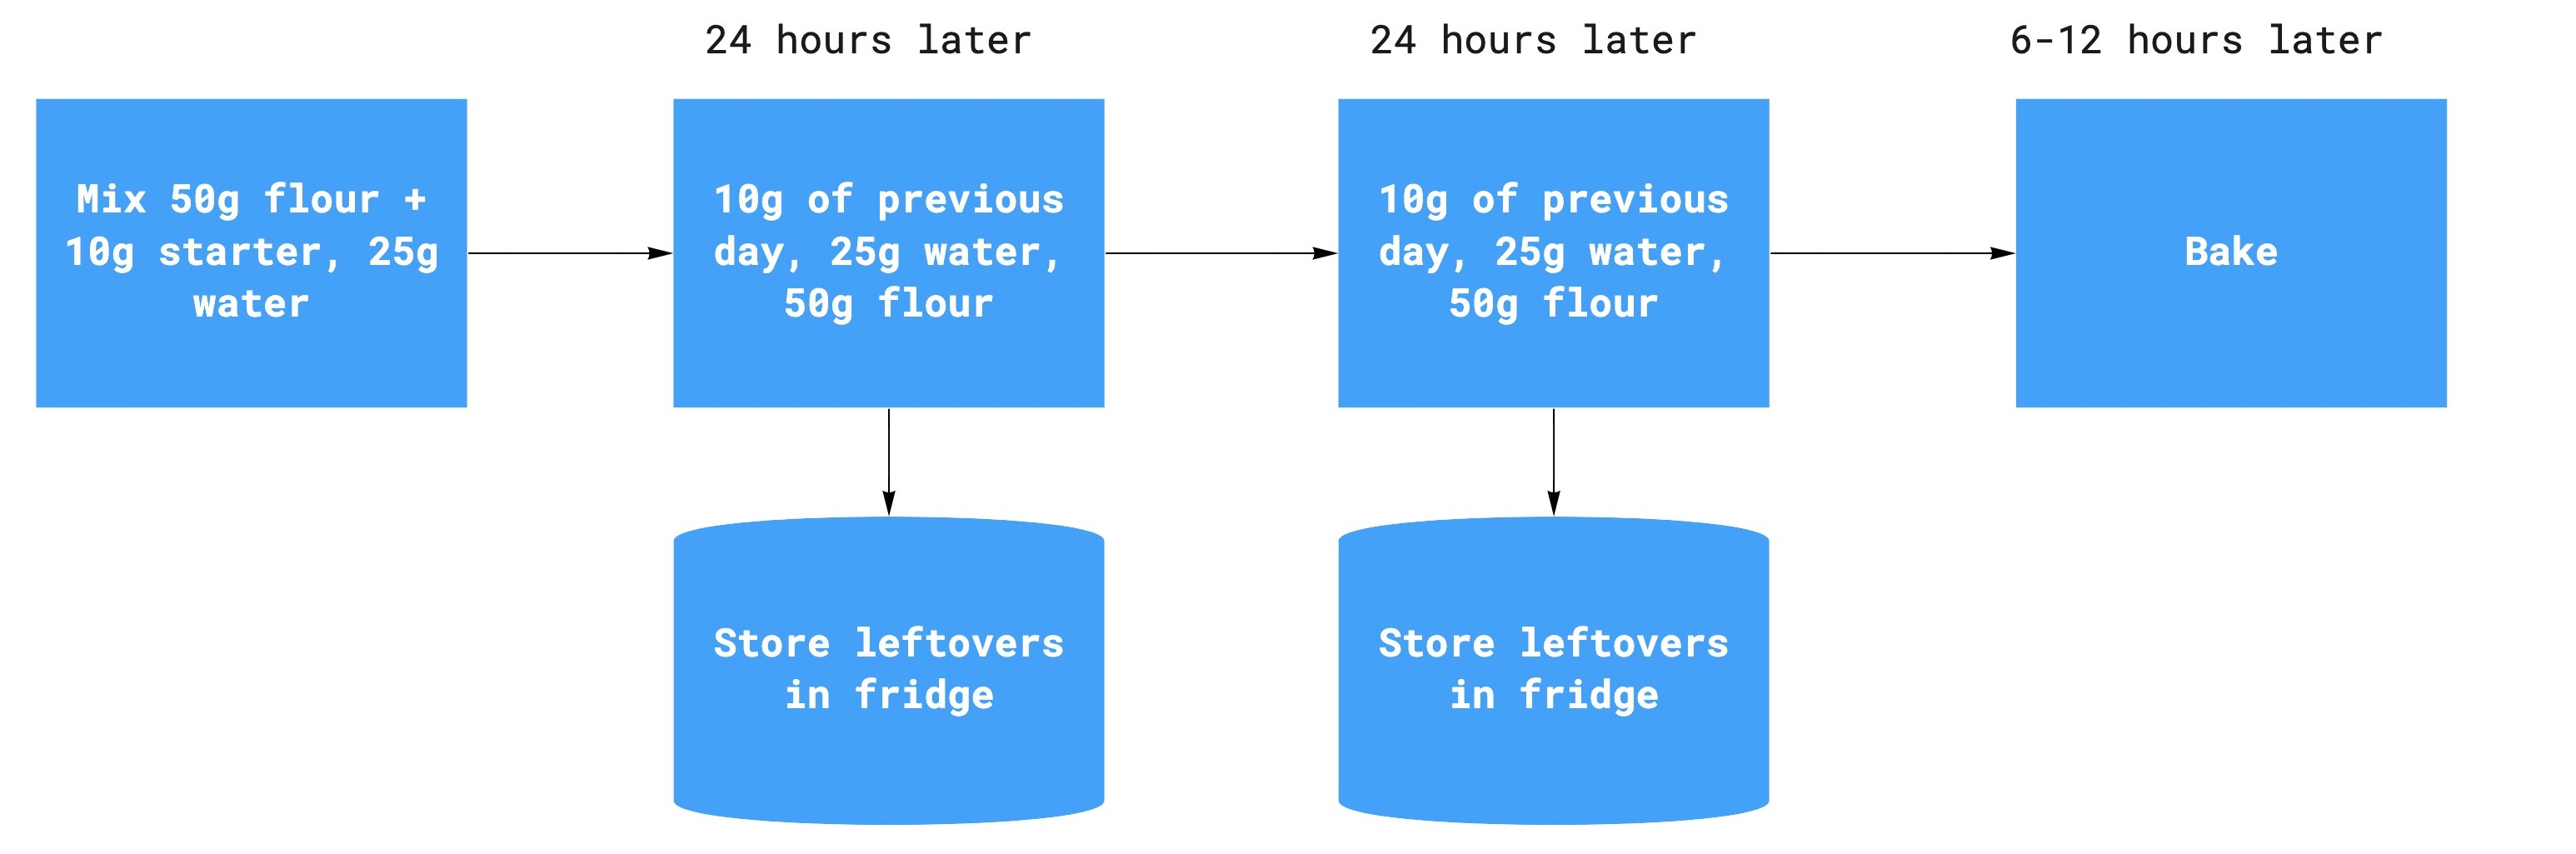
\includegraphics[width=\textwidth]{stiff-starter-conversion}
  \caption{The process to convert your starter into a stiff starter.}
  \label{fig:stiff-starter-conversion}
\end{figure}

Furthermore a stronger flour containing more gluten
will help you to push the fermentation further. This
is because your flour contains more gluten and will
take longer to be broken down by your bacteria. Ultimately
if fermented for too long your dough is also going
to be broken down and will become sticky and flat.

To debug whether the excess bacterial fermentation is the issue,
simply taste your dough. Does it taste very sour? If yes,
that's a good indicator. When working the dough, does it
suddenly become very sticky after a few hours? That's a
another good indicator. Please also use your nose to note
the smell of the dough. It shouldn't be too pungent.

\section{I want more tang in my bread}

To achieve more tang in your sourdough bread you have
to ferment your dough for a longer period of time.
Over time the bacteria will metabolize most of the
ethanol created by the yeast in your dough. The bacteria
mostly produces lactic and acetic acid. Lactic acid
is chemically more sour than acetic acid but sometimes
not achieved as sour. In most cases a longer fermentation
is what you want. You will either need to utilize a loaf
pan to make your dough or use a flour that can withstand
a long fermentation period. A flour like this is typically
called a {\it strong flour}. Stronger flours tend
to be from wheat varieties that have be grown in more
sunny conditions. Because of that stronger flours tend
to be more expensive. For freestanding loaves I recommend
to use a flour that contains at least 12 percent protein.
Generally the more protein the longer you can ferment your dough.

Another option to achieve a more sour flavor could be to
use a starter that produces more acetic acid. Acetic acid
bacteria tend to be more common in rye starters (source needed).
Chemically the acetic acid isn't as sour, but when tasting
it will seem more sour. Make sure to use a starter that is at
a hydration of around 100 percent. Acetic acid production
requires oxygen. A too liquid starter tends to favor lactic
acid production because the flour is submerged in water, no
oxygen can reach the fermentation after a while.

\begin{figure}[!htb]
  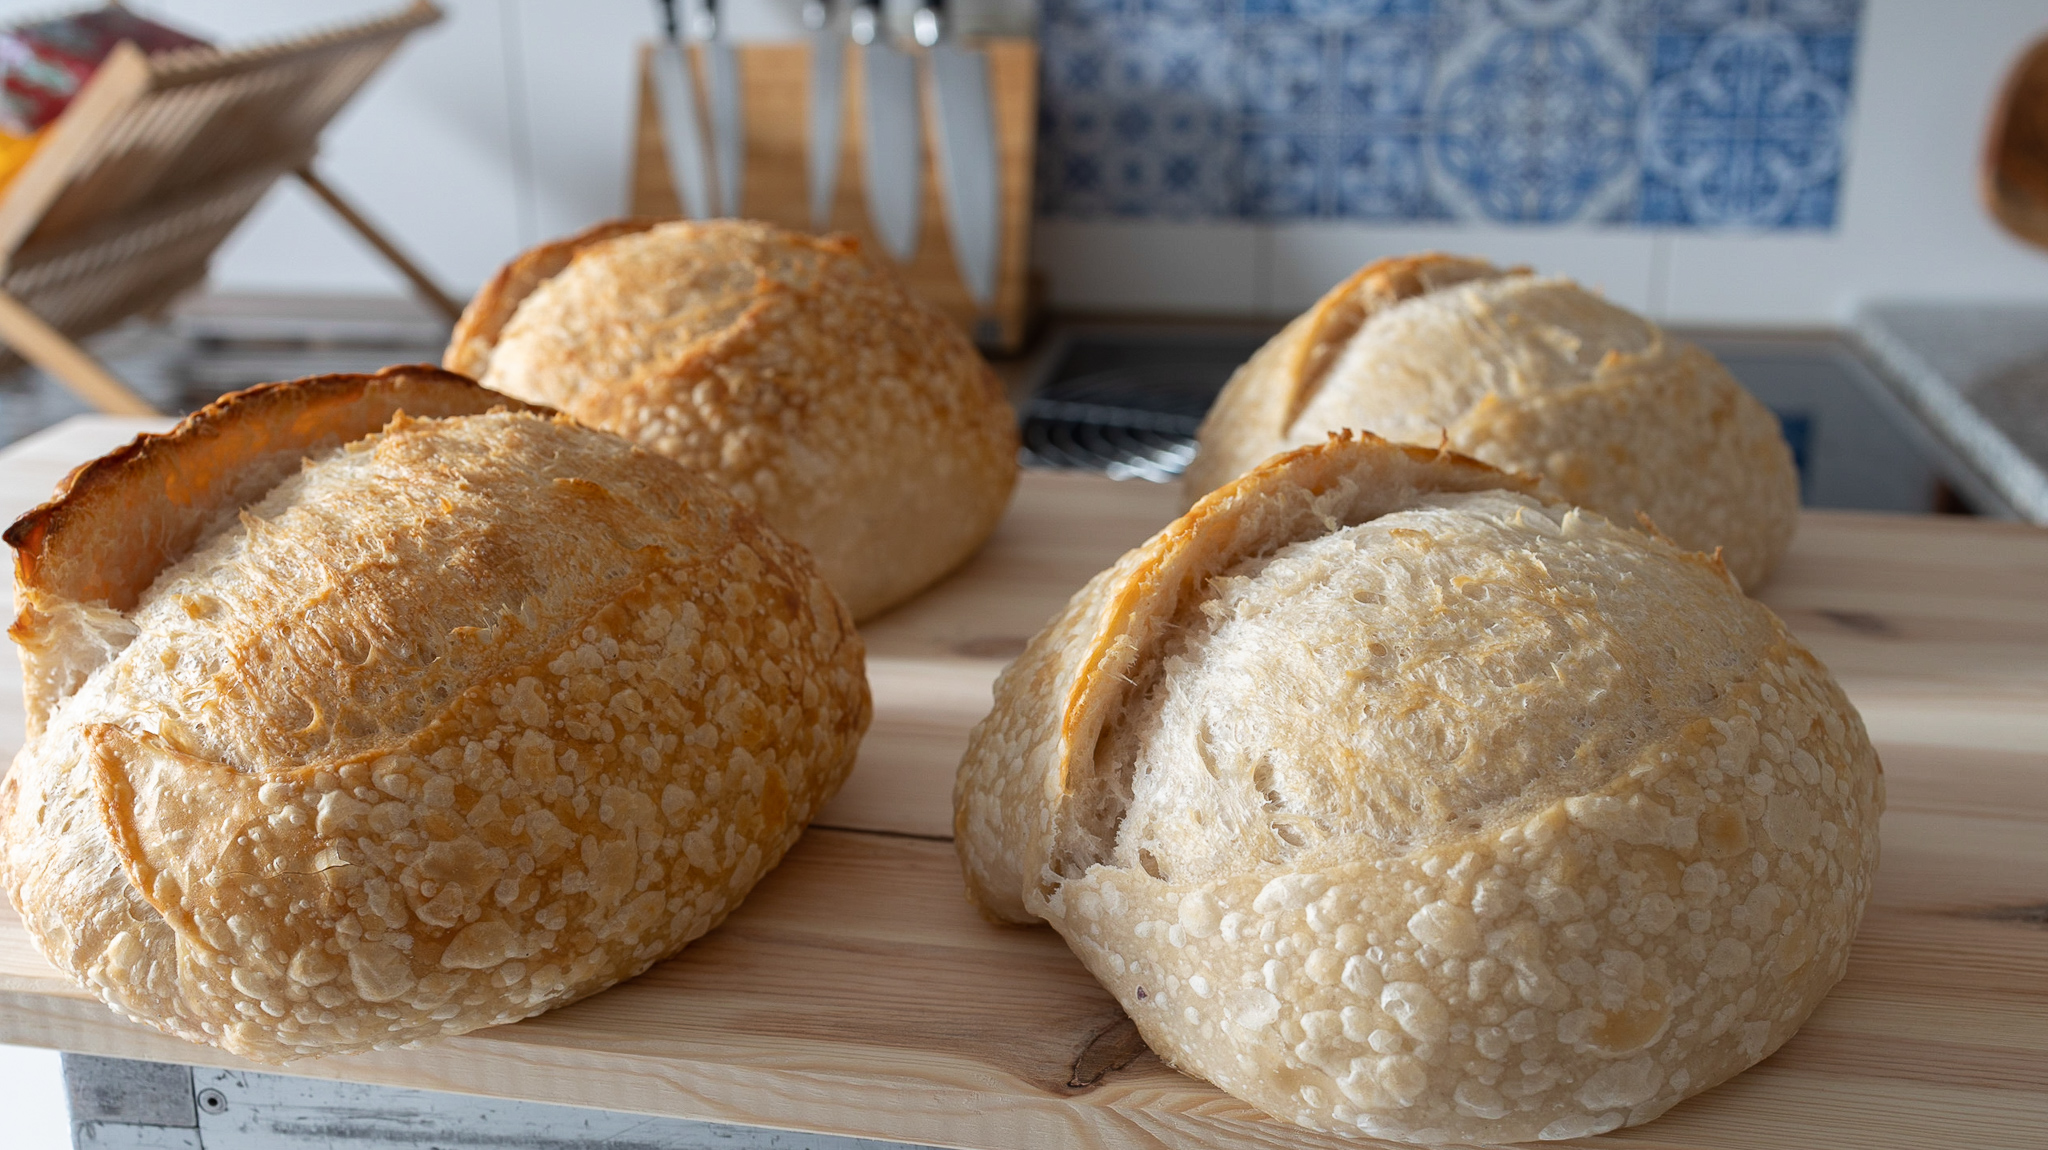
\includegraphics[width=\textwidth]{parbaked-bread.jpg}
  \caption{A half-baked bread, known as "parbaked".}
  \label{fig:parbaked-bread}
\end{figure}

Another more easier option could be to bake your sourdough
twice. I have observed this when shipping bread for my micro
bakery. The idea was to bake my bread for around 30 minutes
until it's sterilized, let it cool down and then ship it
to customers. Once you receive it you just bake it again
for another 20-30 minutes to achieve the desired crust and
then you can eat it. Some of the customers reported a very sour
tasting bread. After investigating a bit more it became
crystal clear. By baking the bread twice you don't boil
as much of the acid during the baking process. Water
evaporates at around 100°C while acetic acid boils at
118°C and lactic acid at 122°c. After baking for 30 minutes
at around 230°C some of the water has started to evaporate,
but not all the acid yet. If you were to continue to bake more
and more of the acid would start to evaporate. Now if you were
to stop baking after 30 minutes, you would typically have reached
a core temperature of around 95°C. Your dough would need
to be cooled down again to room temperature. The crust would
still be quite pale. Then A couple of hours later you start
to bake your dough again. Your crust would become nice and
dark featuring delicious aroma. The aroma is coming from the
maillard reaction. However the core of your dough still won't
exceed the 118°C required to boil the acid. Overall your
bread will be more sour. The enhanced acidity also helps
to prevent pathogens from entering your bread. The bread
will be good for a longer period of time. That's why
the concept of a delivery works well with sour sourdough bread.
In my experiments the bread stayed good for up to a week
in a plastic bag.

\section{My bread is too sour}

Some people like the bread less sour as well. This
is personal preference. To achieve a less sour bread
you need to ferment for a shorter period of time.
The yeast produces CO2 and ethanol. Both yeast and
bacteria consume the sugars released by the amylase enzyme
in your dough. When the sugar is rare bacteria starts to
consume the leftover ethanol by the yeast. Over time more
and more acidity is created making a more sour dough.

Another angle at this would be to change the yeast/bacteria
ratio of your sourdough. You can start the fermentation with
more yeast and less bacteria. This way for the same given
volume increase of your dough you will have less acidity.
A really good trick is to make sure that you feed your starter
once per day at room temperature. This way you shift
the tides of your starter towards a better yeast fermentation \cite*{more+active+starter}.

To shift the tides even further a real game changer
to me has been to create a stiff sourdough starter. The
stiff sourdough starter is at a hydration of around 50 percent.
By doing so your sourdough starter will favor yeast
activity a lot more. Your doughs will be more fluffy and will
not as sour for a given volume increase. I tested this
by putting condoms over different glas jars. I used
the same amount of flour for each of the samples.
I tested a regular starter, a liquid starter and a stiff
starter. The stiff starter by far created the most CO2
compared to the other starters. The balloons were inflated
the most. \cite{stiff+starter}

Another non conventional approach could be to add baking
powder to your dough. The baking powder neutralizes the
lactic acid and will make a much milder dough.\cite{baking+powder+reduce-acidity}

\section{Fixing a moldy sourdough starter}

First of all - making a moldy sourdough starter is very difficult.
It's an indicator that something might be completely off in your starter.
Normally the symbiosis of yeast and bacteria does not allow external
pathogens such as mold to enter your sourdough starter.
The low pH created by the bacteria is a very hostile environment
that no other pathogens like. Generally everything below a pH
of 4.2 can be considered food safe\cite{food+safe+ph}. This
is the concept of pickled foods. And your sourdough bread
is essentially pickled bread.

I have seen this happening especially when the sourdough
starter is relatively young. Each flour naturally contains
mold spores. When beginning a sourdough starter all
the microorganisms start to compete by metabolizing the
flour. Mold can sometimes win the race and out compete
the natural wild yeast and bacteria. In that case simply
try cultivating your sourdough starter again. If it molds
again it might be a very moldy batch of flour. Try a different
flour to begin your sourdough starter with.

Mature sourdough starters should not mold unless the conditions
of the starter change. I have seen mold appearing when the starter is stored
in the fridge and the surface dried out. Also sometimes on the
edges of your starter's container. Typically in areas where no active
starter microorganisms can reach. Simply try to extract an
area of your starter that has no mold. Feed it again with flour and
water. After a few feedings your starter should be back to normal.
Take only a tiny bit of starter. 1-2 grams are enough. They already
contain millions of microorganisms.

Mold favors aerobic conditions. This means that air is required in order
for the mold fungus to grow. Another technique that has worked for me
was to convert my sourdough starter into a liquid starter. This successfully
shifted my starter from acetic acid production to lactic acid production.
Acetic acid similarly to mold requires oxygen to be produced. After
submerging the flour with water over the time the lactic acid bacteria
out competed the acetic acid bacteria. This is a similar concept to pickled
foods. By doing this you are essentially killing all alive mold fungi. You
might only have some spores left. With each feeding the spores will become
less and less. Furthermore it seems that lactic acid bacteria produce
metabolites that inhibit mold growth. \cite{mold+lactic+acid+bacteria}

\begin{figure}[!htb]
  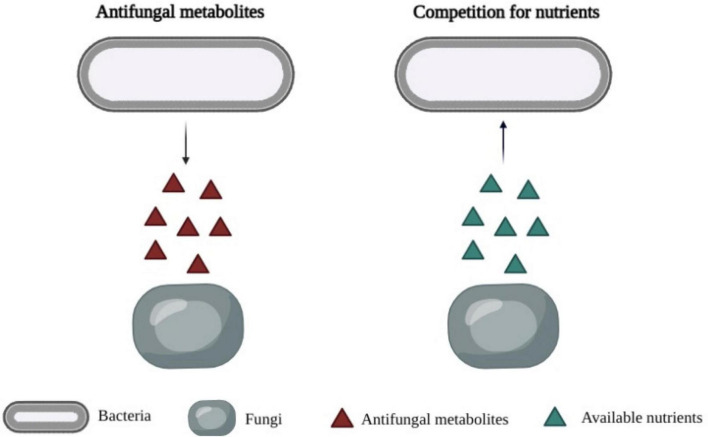
\includegraphics[width=\textwidth]{fungi-lactic-acid-interactions}
  \caption{The interaction of lactic acid bacteria and mold fungi.
           The authors Ce Shi et al. show how bacteria are producing
           metabolites that inhibit fungus growth. \cite{mold+lactic+acid+bacteria}}
  \label{fig:fungi-lactic-acid-interactions}
\end{figure}

To pickle your starter simply take a bit of your existing starter (5 grams for
instance). Then feed the mixture with 20g of flour and 100g of water. You have
created a starter a hydration of around 500 percent. Shake the mixture vigorously.
After a few hours you should start seeing most of the flower near the bottom
of your container. After a while most of the oxygen from the bottom mixture
is depleted and anaerobic lactic acid bacteria will start to thrive. Take a
note of the smell your sourdough starter. If it was previously acetic
it will now change to be a lot more dairy. Extract a bit of your mixture the
next day by shaking everything first. Take 5g of the previous mixture, feed
again with another 20g of flour and another 100g of water. After 2-3
additional feedings your starter should have adapted. When switching back
to a hydration of 100 percent the mold should have been eliminated. Please note that
more tests should be conducted on this topic. It would be nice to really
carefully analyze the microorganisms before the pickling and after.

\section{My bread flattens out removing it from the banneton}

After removing your dough from the banneton your dough will always
flatten out a bit. That's because over time your gluten network
relaxes and can no longer hold the shape. However, during the course
of baking your dough is going to increase in size and inflate again.

If your dough however flattens out completely it's a sign that
you have fermented your dough for too long. Please refer to ~\ref{sec:overfermented-dough}
where I explain about overfermented doughs. Your bacteria
has consumed most of your gluten network. That's why your
dough fully collapses and stays flat during the bake. The
CO2 and evaporating water will diffuse out of the dough.
A related symptom is that your dough sticks to the banneton.
When starting baking I combatted this with rice flour.
It works but might be a false friend. I gently rub my
dough with a bit of non-rice flour before placing it in
the banneton. Now then the dough starts to stick to the banneton
while I remove it I resort to a drastic measure. I immediately
grease a loaf pan and directly place the dough inside. The loaf
pan provides a barrier and the dough can't flatten out as much.
The dough won't be as fluffy but super delicious if you love tangy bread.

If you own a pH meter take a note of your dough's pH before baking.
This will allow you to better judge your dough throughout
the fermentation process.

\section{My bread flattens out during shaping}

Similarly to a dough flattening out after removing it from the banneton,
a flattened dough after shaping is also a possible sign of overfermentation.

When you try to shape the dough, can you easily tear pieces from the dough?
If yes, you have definitely overfermented your dough. If not it might just
be a sign that you have not created enough dough strength for your dough.
A ciabatta for instance is a dough that tends to flatten out a bit after shaping.

If your dough is not possible to be shaped at all use a greased loaf pan
to rescue your dough. You can also cut a piece of the dough and use it
as the starter for your next dough. Your sourdough dough is essentially
just a gigantic starter.

\section{Liquid on top of my starter}

Sometimes a liquid in many cases black liquid gathers on top
of your sourdough starter. The liquid might have a pungent
smell to it. Many people confuse this with mold. I have seen
bakers recommending to discard the starter because of this liquid.
The liquid is commonly known as {\it hooch}. After a while
of no activity the heavier flour separates from the water. The flour
will sit at the bottom of your jar and the liquid will stay on top.
The liquid turns darker because some particles of the flour weigh
less than the water and float on top. Furthermore dead microorganisms
float in this liquid. This liquid is not a bad thing, it's actively
protecting your sourdough starter from aerobic mold entering through
the top.

\begin{figure}[!htb]
  \centering
  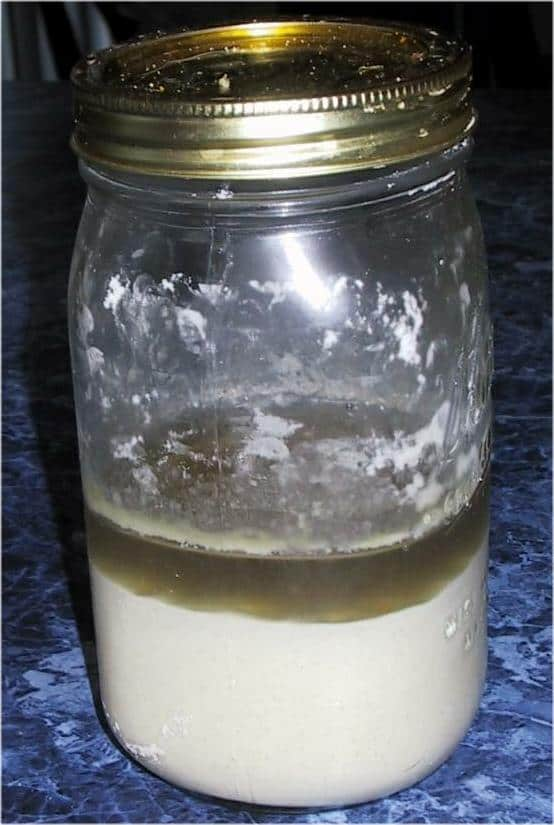
\includegraphics[width=0.5\textwidth]{hooch}
  \caption{Hooch building on top of a sourdough starter. \cite{liquid+on+starter}}
  \label{fig:hooch}
\end{figure}

Simply stir your sourdough starter to homogenize the hooch back
into your starter. The hooch will disappear. Then use a little bit of
your sourdough starter to setup the starter for your next bread.
Once hooch appears your starter has likely fermented for a long
period of time. It might be very sour. This state of starter
is excellent to make discard crackers or a discard bread. Don't throw
anything away. Your hooch is a sign that you have a long fermented
dough in front of you. Compare it to a 2 year ripened Parmigiano cheese.
The dough in front of you is full of delicious flavor.

\section{Why does my starter smell like vinegar or acetone?}

Your sourdough starter has likely produced a lot of acetic acid.
Acetic acid is essential when creating vinegar. Once no additional
food is left some of your starter's bacteria will consume ethanol
and convert it into acetic acid. Acetic acid has a very pungent smell.
When tasting acetic acid the flavor of your bread is often perceived
as quite strong.

\begin{figure}[!htb]
  \centering
  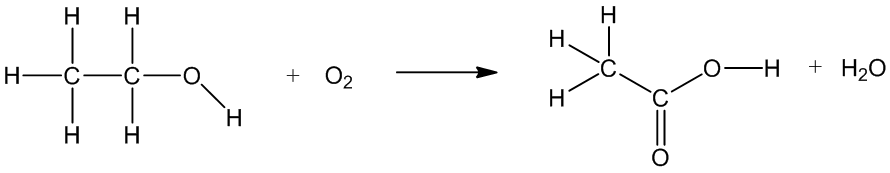
\includegraphics[width=1.0\textwidth]{ethanol-oxidation}
  \caption{Oxygen is required to create acetic acid \cite{acetic+acid+production}.}
  \label{fig:ethanol-oxidation}
\end{figure}

This is nothing bad. But in case you would like to change
the flavor of your final bread consider converting
your sourdough starter into a liquid starter. This will
help to prioritize lactic acid producing bacteria.
Your flavor will change to dairy compared to vinegary.
You can't go back though. After the conversion your starter
will never go back to acetic acid production because you have
changed the tides towards primarily lactic acid fermentation.
I like to have a separate rye starter. In my experiments
rye starters tend to feature many acetic acid bacteria.
This starter is excellent when you want to make a very hearty
strong tasting bread. A pure rye bread tastes excellent when
made with such a starter. The flavor when taking a bite
is incredible. It nicely plays with soups as well. Just take
a bit of this bread and dip it in your soup.

\section{My crust becomes chewy}

Depending on which style of bread you are making a
thick crackly crust is sometimes desired. The crust
of your bread is created during the 2nd stage of the
baking process once the steaming source of your
oven has been removed. The dark colors are created by
the process known as {\it Maillard reaction} and then followed
by another process known as {\it caramelization}. Each
color of crust offers the taster a different aroma.

What happens quite often is that the crust becomes chewy after a day.
Sometimes when baking in the tropics with high humidity the
crust only stays in this stage for a few hours. Afterwards
the crust becomes chewy. It's no longer as crisped compared
to the moment after baking. Your dough still contains moisture.
This moisture will start to homogenize in the final bread and
partially evaporate. The result is that your crust becomes chewy.

Similarly when storing your bread in a container or in a plastic
bag your crust is going to become chewy. I have no fix for this yet.
I typically tend to store my breads in a plastic bag inside of my fridge.
This allows the moisture to stay inside of bread. When taking a slice
I always toast each slice. This way some of the crispness returns.
If you know of a great way please reach out and I will update
this book with your findings.

\printbibliography


\end{document}